\chapter{Results}
\label{chap:results}
\begin{comment}
Results
Some plots
Rewards - loss - RMSE

We choose some models, to reflect the \textbf{hyperparameters} choices (Magnus does reward). Use "best performance" regardless of number of runs and 

Summarise best results, based on hyperparameters and under what controls (reward, goal setting, rules idk) also vs. the baseline (paper or OpenAI release) implementation. 

Do this separately for DDPG and PPO, internal competition, then compare best of the two. 

Can we generalise results based on some hyperparameters? Can we come to conclusions on others? Don't over-complicate. 

3 robustness tests for PPO, 2 for DDPG
Results in excel,
\end{comment}

\section{Overview}

In this chapter, we will present the results for the DDPG and PPO algorithms. This will include a presentation of some of the selected models for each algorithm, where we look at the effect of hyperparameters in the training process and the overall performances during testing. Lastly, the best models are tested again with $\pm10\%$ mass to evaluate their robustness.

To visualise the results, we have the training graphs for each model. These include one for \textit{average return}, \textit{actor loss} and \textit{critic loss}. The average return will be our standard performance metric for the agent, while the loss analysing the loss curves will provide information about the actor-critic networks. We also provide the model training times, run on an Intel(R) Core(TM) i7-8700 CPU @ 3.20GHz processor.

For the fixed waypoint tests, a goal point is initialised at roughly $[1.84, 1.84, 1.5]$ meters away, or exactly at a point with $r=3$m with relative angles $\psi=45\degree$ and $\theta = -30\degree$. 
\begin{figure}[hbt]
    \centering
    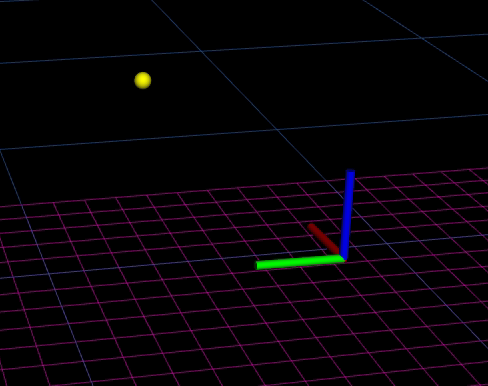
\includegraphics[scale=0.8]{figures/5_/5_waypoint.png}
    %\captionsetup{justification=centering}
    \caption{The goal seen with a yellow marker with $\p_0 = \approx [1.84, 1.84, 1.5]$.The quadrotor body frame is shown as \textcolor{red}{x}, \textcolor{green}{y}, \textcolor{blue}{z}.}
    \label{fig:5_waypoint}
\end{figure}
This is calculated through $x = r \sin{\theta}  \cos{\psi}, \,\,y = r \sin{\theta}  \sin{\psi}$ and $z = r \cos{\theta}$.

With this, each model will then attempt to fly to this goal marker 100 times and we compute the root-mean-squared cross-track error (RMSE) and average return per episode, averaged across all episodes. The cross-track error is calculated by finding the perpendicular distance to the quadrotor from a point on the shortest path (line) to the goal.
Additionally, for select scenarios we distinguish models further by plotting a typical run, such that we can see the quadrotor flight trajectories and can analyse its response.

\section{DDPG}
\label{sec:5_DDPG}

The DDPG models chosen for testing are shown in Table \ref{table:4_6_DDPG_hyperparameters}.
\begin{table}[hbt]
    \centering
    \begin{tabular}{||M{3.5cm}||M{3cm}|M{3cm}|M{2cm}||}
    \hline
    \centering
    Model & Network size & Learning rate, $\alpha$ & Buffer size \\ \hline\hline
    Previous NTNU & 64, 64       & 1e-5, 1e-5                           & 1e5            \\ \hline
    Original & 200, 100     & 1e-4, 1e-3                           & 1e6            \\ \hline
    Modified & 64, 64       & 1e-4, 1e-3                           & 1e5            \\ \hline
    \end{tabular}
    \caption{The different DDPG models tested, along with their hyperparameters. The size 200, 100 refers to the sizes of the first and second hidden layers, while the rate 1e-4, 1e-3 are the learning rates for the critic and actor respectively.}
    \label{table:4_6_DDPG_hyperparameters}
\end{table}
To explain the names, the ``Previous NTNU'' model is the model that was implemented in previous projects here at NTNU, while the ``Original'' one denotes the baseline implementation by \cite{DDPG}. In addition, the ``Modified'' model is chosen to illustrate a good combination of hyperparameters from the Previous NTNU and Original models.

\subsection{Training}
\label{sec:5_ddpg_training}
The training of these models are done as described in Section \ref{sec:4_5_trainingSetup}. For DDPG, we found that the models required a significant amount of training time to achieve a good performance.
\begin{table}[hbt]
    \centering
    \begin{tabular}{||M{3cm}|M{3cm}|M{4cm}||}
    \hline
    \centering
    Model & Epoch & Training time \\ \hline\hline
    NTNU     & 1452 & 18h 4m  \\ \hline
    Original & 1792 & 21h 25m \\ \hline
    Modified & 1500 & 17h 44m \\ \hline
    \end{tabular}
    \caption{The time used to train each of the DDPG models presented.}
     \label{table:5_trainingTime_DDPG}
\end{table}
We have selected the last epoch as the best epoch for each of these models, based from the training curves seen in Figure \ref{fig:5_training_DDPG}.
\begin{figure}[H]
     \centering
     \begin{subfigure}[b]{0.78\textwidth}
         \centering
         \captionsetup{justification=centering}
         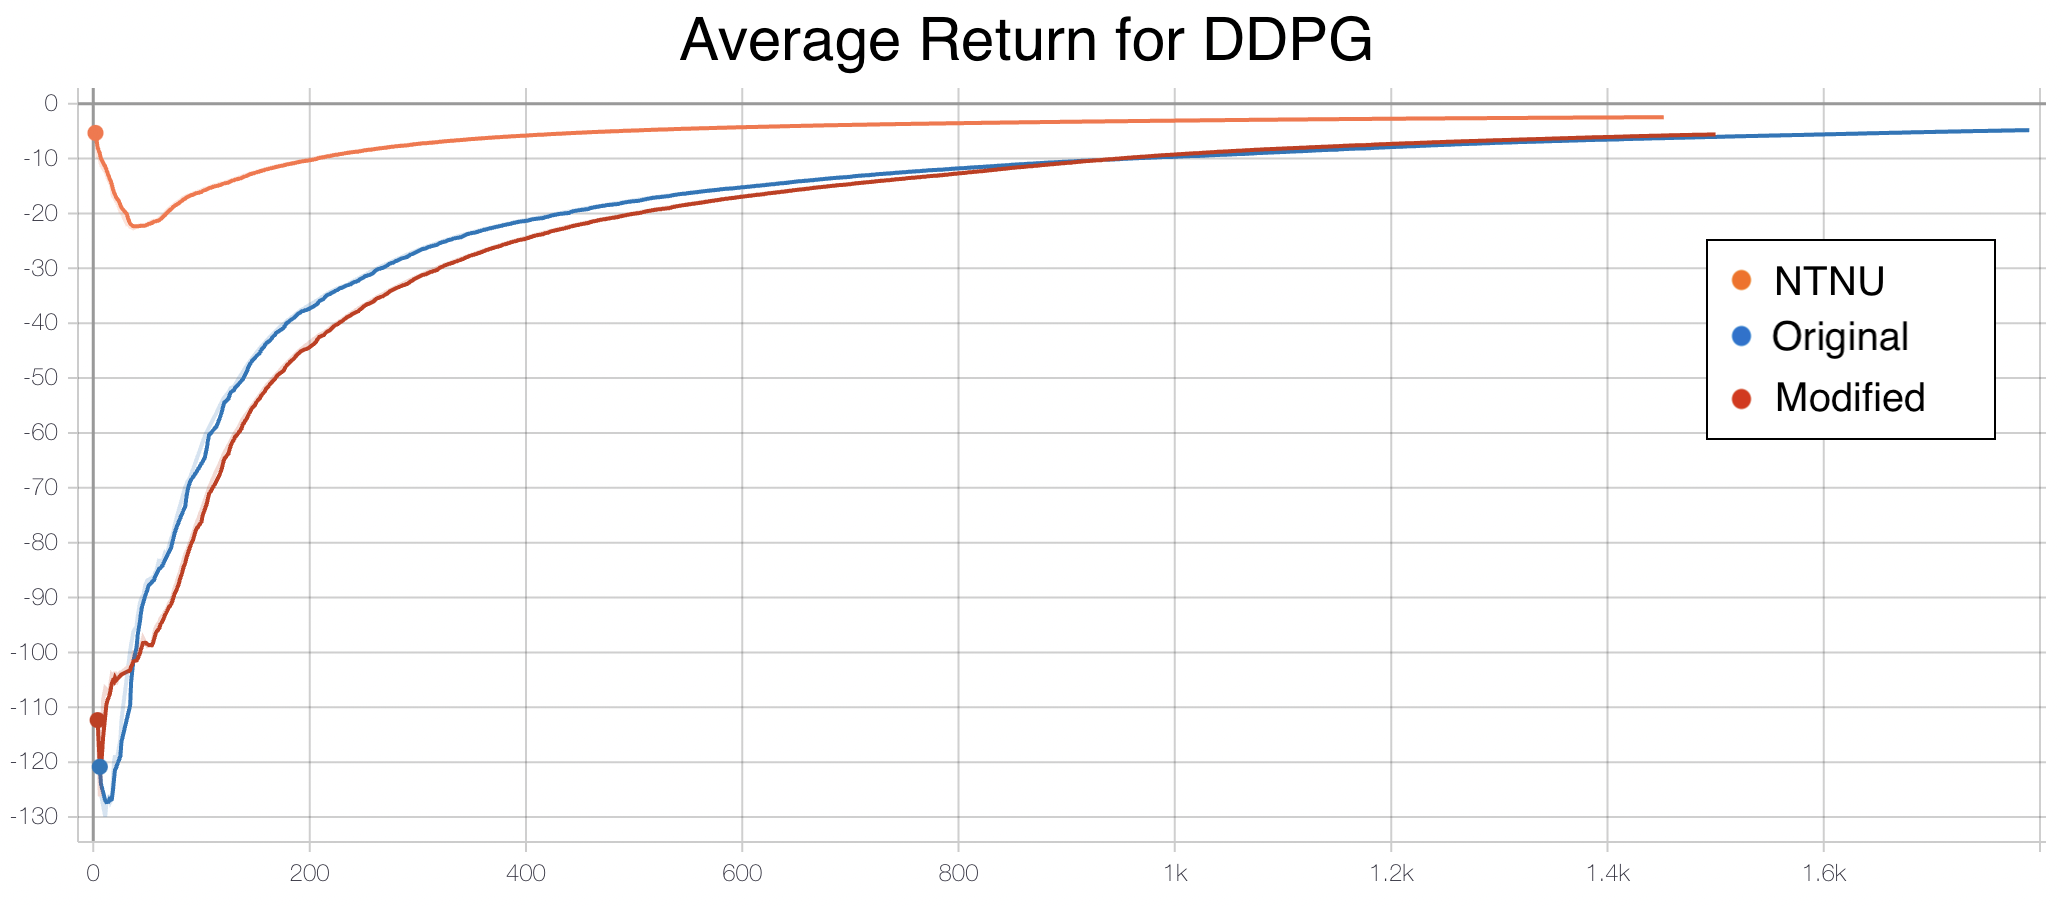
\includegraphics[width=\textwidth]{figures/5_/Training/ddpg_return.png}
         \caption{Average return for the three DDPG models, where the return is averaged across all previous episodes.}
         \label{fig:training_ddpgReturn}
     \end{subfigure} 
     \hfill \\[5mm]
     \begin{subfigure}[b]{0.78\textwidth}
         \centering
         \captionsetup{justification=centering}
         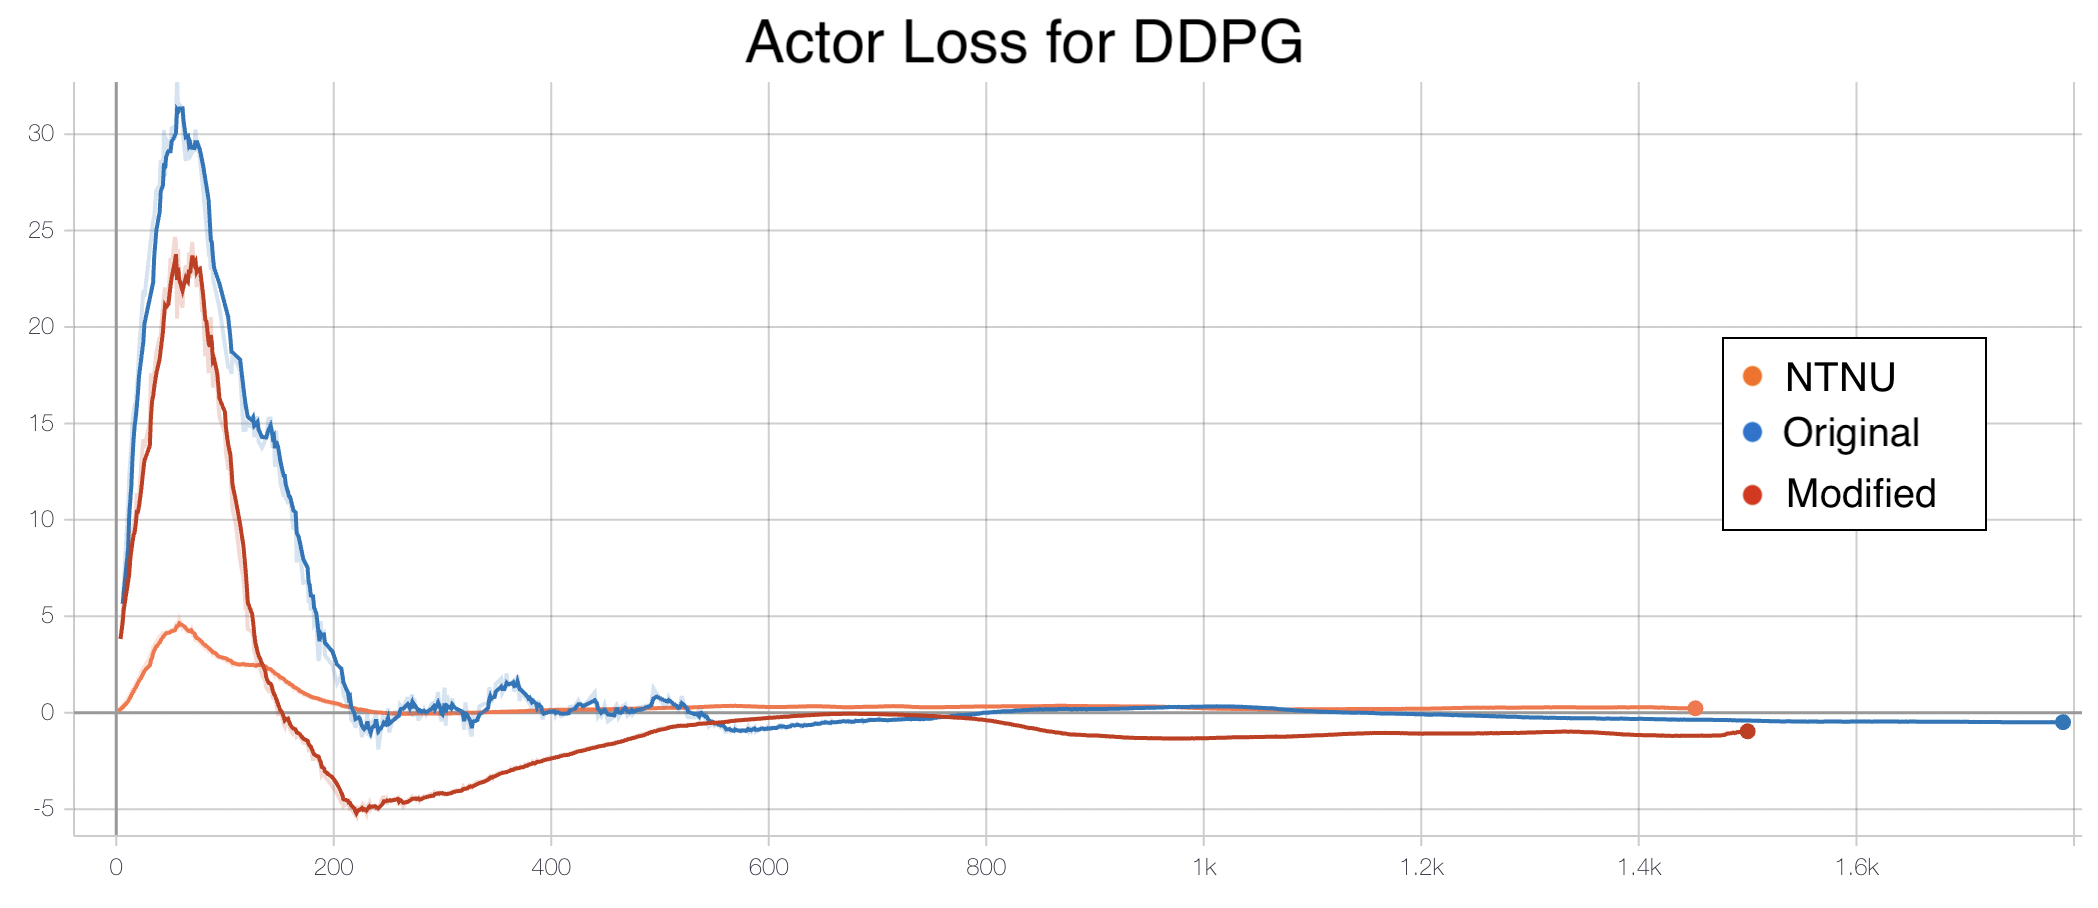
\includegraphics[width=\textwidth]{figures/5_/Training/ddpg_actorLoss.png}
         \caption{The actor loss of the DDPG models per epoch, given by the \textit{negative} of the actor objective function, $\Qt$, as seen in Equation \eqref{3_4_actorLoss}.}
         \label{fig:training_ddpgActorLoss}
     \end{subfigure}
     \hfill \\[5mm]
     \begin{subfigure}[b]{0.78\textwidth}
         \centering
         \captionsetup{justification=centering}
         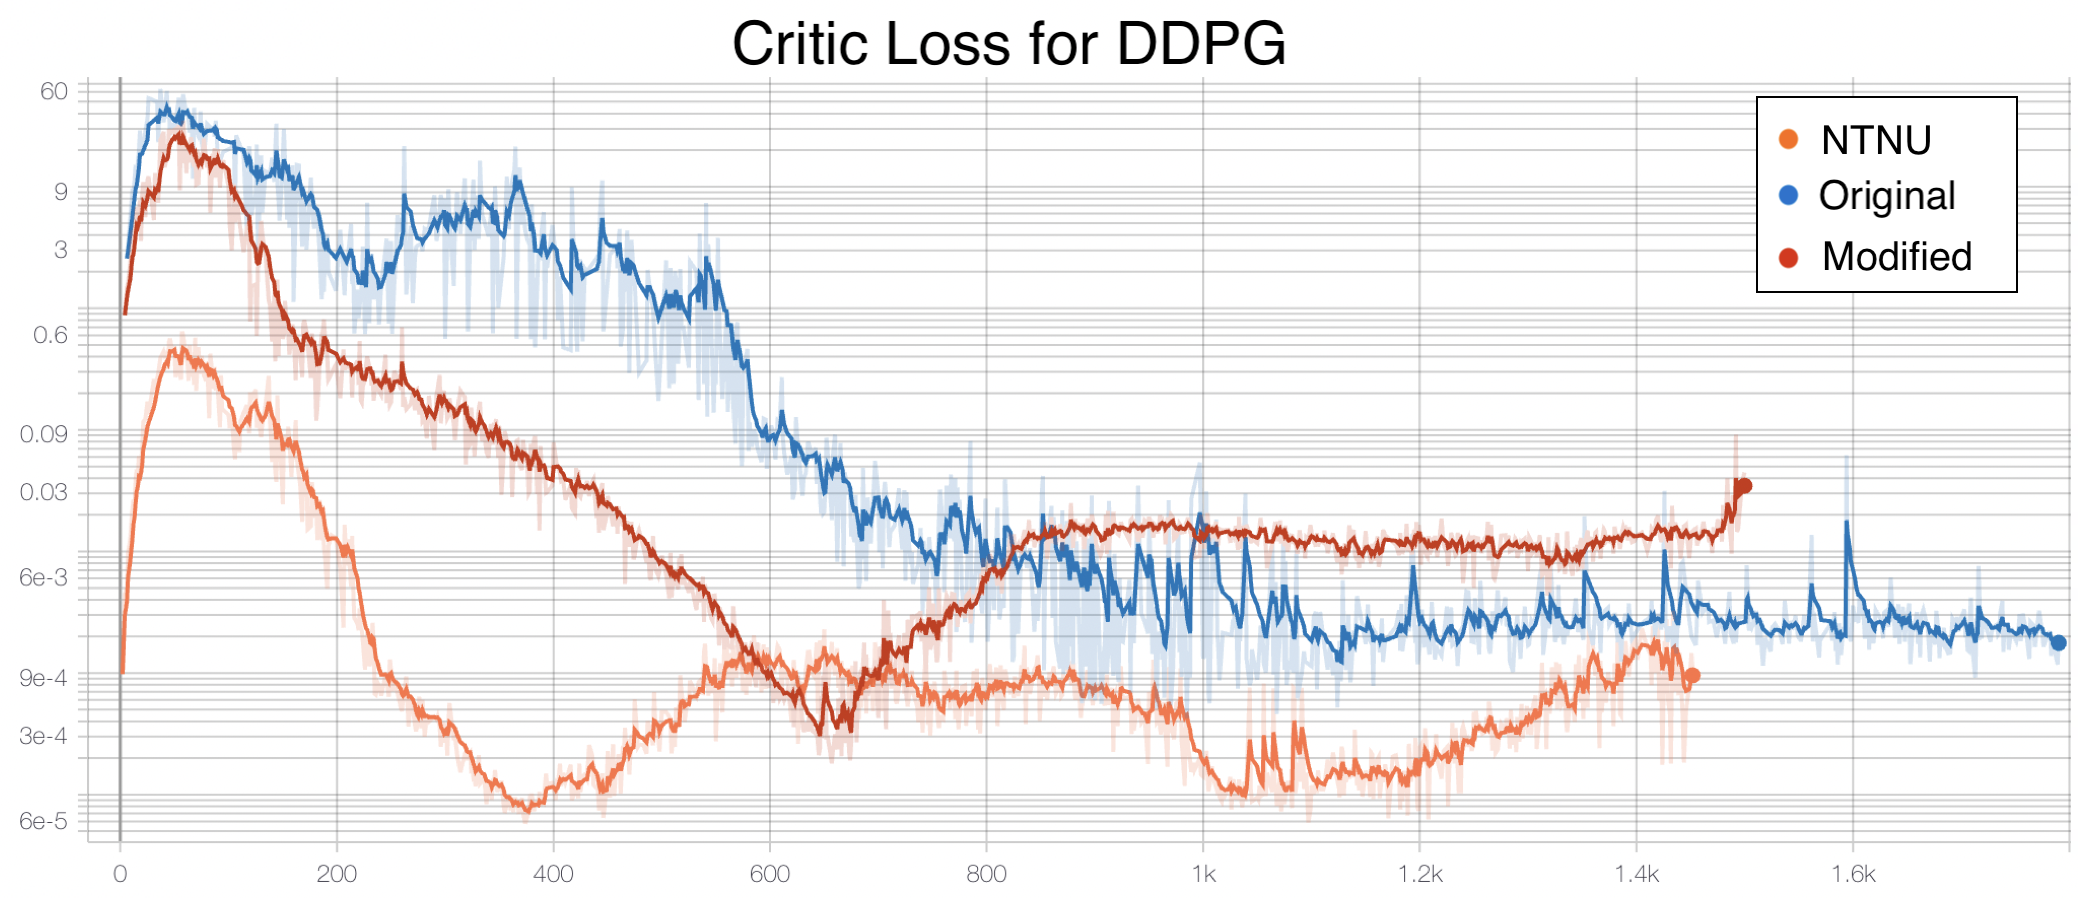
\includegraphics[width=\textwidth]{figures/5_/Training/ddpg_criticLoss.png}
         \caption{The critic loss of the DDPG models per epoch. The loss is the MSE of the estimated Q-value and the target Q-value, shown in Equation \eqref{3_4_criticLoss}. Note the log $y$-axis.}
         \label{fig:training_ddpgCriticLoss}
     \end{subfigure}
    \captionsetup{justification=centering}
    \caption{The training process for the three DDPG models. The $x$-axis shows the number of epochs the model is trained for where an epoch is 20 episodes.}
     \label{fig:5_training_DDPG}
\end{figure}
Looking at the Figure \ref{fig:5_training_DDPG}, we observe that the Previous NTNU model has the highest average return, with the Original and Modified models practically identical. For reference, at the end of their training, each model had an average return of -2.45, -4.80, -5.58 respectively.
We should also note that the average return curve is surprisingly smooth. This is because the average return is the mean return over all previous episodes and not the 20 episodes of that particular epoch. Arguably, this could be a design flaw in hindsight. So knowing this, the actual value of the average return for a certain epoch may be misleading of the agent's performance, and actually, it is not clear to see which model is performing best amongst the three. 

Therefore, we can instead look at the actor-critic loss curves. Beginning first with the actor loss in Figure \ref{fig:training_ddpgActorLoss}, we can see that by roughly 700 epochs all the values settle at 0. However, we then see that both the Modified and the Original loss curves converge to negative loss values, which initially might appear strange if we think about its definition (describing a negative error?).
Yet, since the actor loss is actually just the \textit{negative} of the estimated return $\Qt$, we should understand the actor loss as DDPG's method of predicting the actor performance. This makes sense since a high actor loss means very negative expected return and bad performance, while a low actor loss means high expected return which is a good performance. 

However, the $\Qt$ value is merely a prediction. To gauge its accuracy, we turn to the critic loss. Given by Equation \eqref{3_4_criticLoss}, the critic loss is the MSE of the target Q-value and its current prediction, corresponding to the prediction error $\overline{VE}$ in Section \ref{sec:3_3_actor-critic}. 
So, as the critic loss approaches 0, the target critic and critic networks essentially are in agreement throughout the episode, which only happens if DDPG does well to predict its Q-value for each state of the episode. So, this is means that a \textit{low critic loss} is an indication of consistently \textit{accurate critic Q-value} predictions.
From Figure \ref{fig:training_ddpgCriticLoss}, we see that all critic losses approach 0 relatively quickly, such that by epoch 750 all losses are below 0.01.
From epoch 800 onwards, the losses flatten, which shows low rates of learning and is a good indication that we can trust the Q-values. 

This means that by reading the actor loss again, we see that from epoch 1000, the best model is in fact the Modified model, which predicts the highest (negative) average return for each epoch. Then the Original model follows second, which has a higher estimated return compared the Previous NTNU model, seen at epoch 1500.
As for the hyperparameters, we can attribute the difference in training largely to the significantly larger learning rates, which transforms the worst model, the Previous NTNU one, into the best model in roughly the same amount of training epochs. We also note that having a larger network size and buffer size does not improve training in this example, though this is not conclusive.

\subsection{Testing}
\label{sec:5_ddpg_tests}
Now that we analysed the training data of these models, we can now test these models and see if the test data concurs with our analysis. The results for our three models on the fixed goal task is given in Table \ref{table:5_DDPG_tests}.
\begin{table}[hbt]
    \centering
    \begin{tabular}{||M{2cm}||M{2.5cm}|M{3.5cm}|M{2.5cm}||}
    \hline
    Model & Goal Rate & Average Return & Average RMSE \\\hline\hline
    NTNU     & 0      & -6.539     & 0.170    \\\hline
    Original & 96      & -0.040     & 0.042    \\\hline
    Modified & 98      & -0.704     & 0.029 \\\hline
    \end{tabular}
    \caption{The test results for the DDPG models, averaged over 100 episodes.}
    \label{table:5_DDPG_tests}
\end{table}

From this table, we observe that the Modified model reached the goal most often at 98\% success, followed by the Original at 96\%. We also note that the Previous NTNU model was not able to reach the goal at all at its point in training. We also see from the Modified model is consistently taking the shortest path to goal among the three models, seen through the low RMSE. 

Very unexpectedly, however, we observe that the average return for the Modified model is much less than the Original model, contradicting the results of the goal rate and average RMSE. To know for sure, we can take a look at the last test run for both models in Figure \ref{fig:5_testing_DDPG}.
\begin{figure}[H]
     \centering
     \begin{subfigure}[b]{0.51\textwidth}
         \centering
         \captionsetup{justification=centering}
         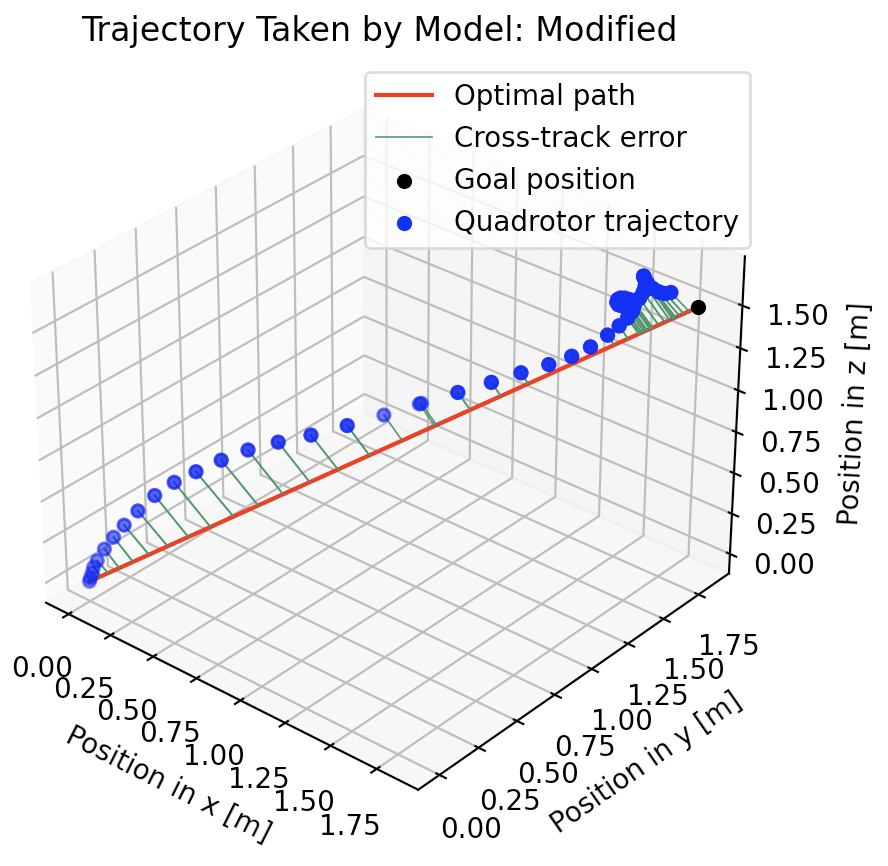
\includegraphics[width=\textwidth]{figures/5_/Testing/ddpg_test_modified1.png}
         \caption{The trajectory of the quadrotor with the Modified model compared to the shortest path.}
         \label{fig:testing_ddpgModified1}
     \end{subfigure} 
     \hfill 
     \begin{subfigure}[b]{0.48\textwidth}
         \centering
         \captionsetup{justification=centering}
         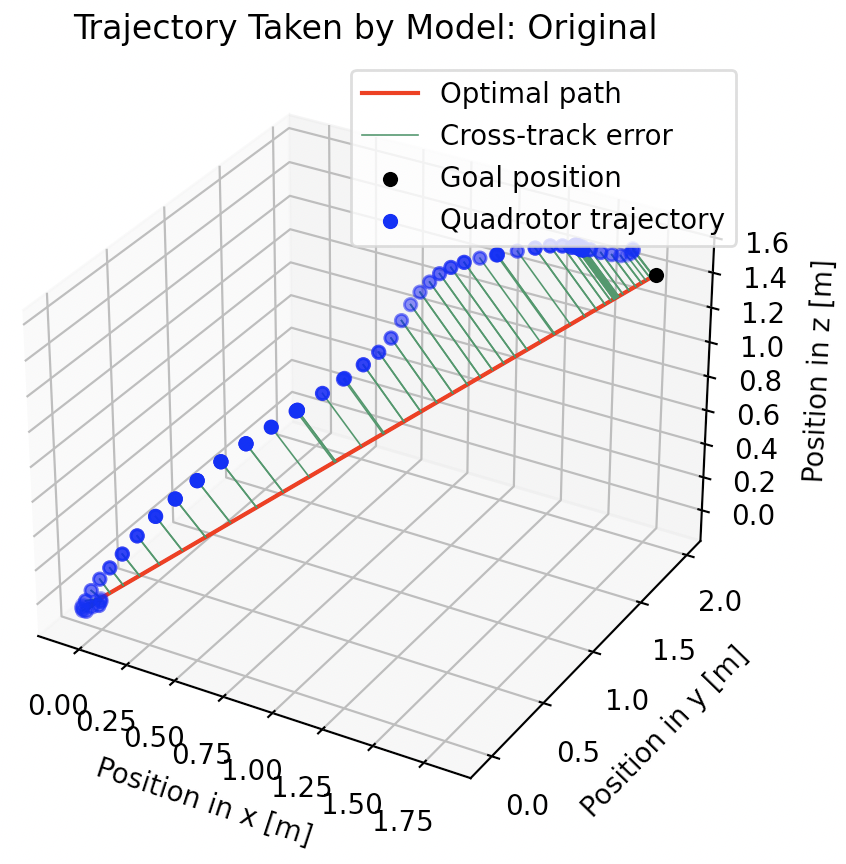
\includegraphics[width=\textwidth]{figures/5_/Testing/ddpg_test_original1.png}
         \caption{The trajectory of the quadrotor with the Original model compared to the shortest path.}
         \label{fig:testing_ddpgOriginal1}
     \end{subfigure} 
     \hfill \\[10mm]
     \begin{subfigure}[b]{0.49\textwidth}
         \centering
         \captionsetup{justification=centering}
         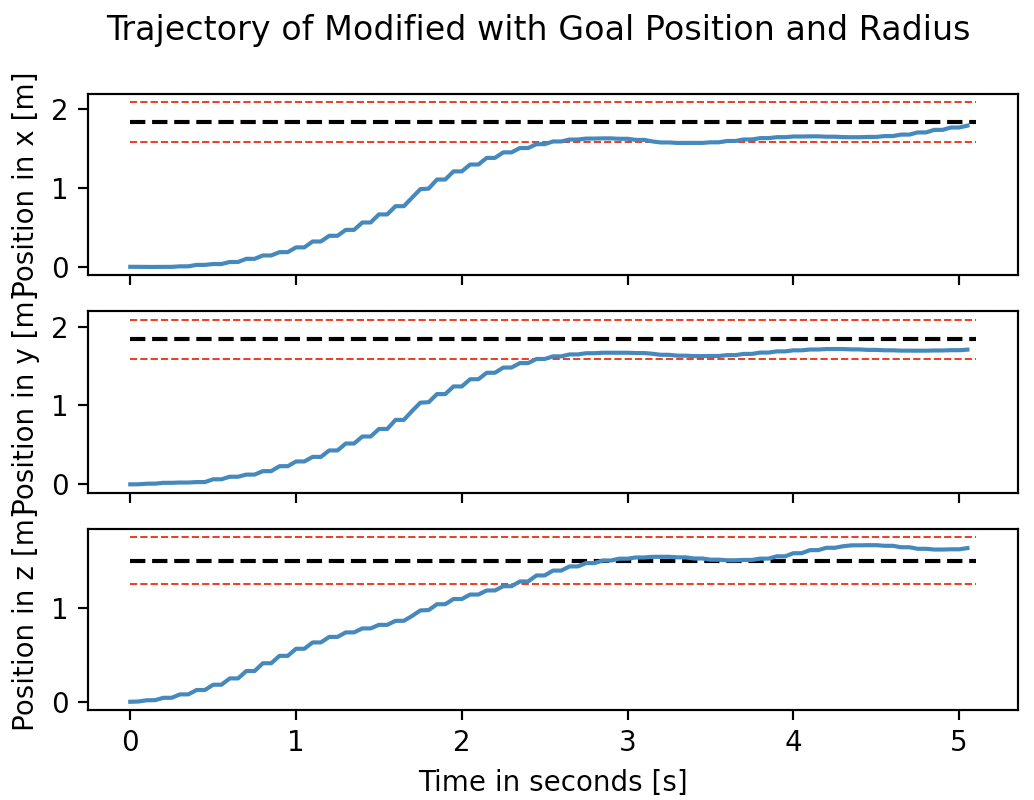
\includegraphics[width=\textwidth]{figures/5_/Testing/ddpg_test_modified2.png}
         \caption{The trajectory of the quadrotor with the Modified model compared to the goal position, decomposed in $x$, $y$, $z$.}
         \label{fig:testing_ddpgModified2}
     \end{subfigure} 
     \hfill 
     \begin{subfigure}[b]{0.49\textwidth}
         \centering
         \captionsetup{justification=centering}
         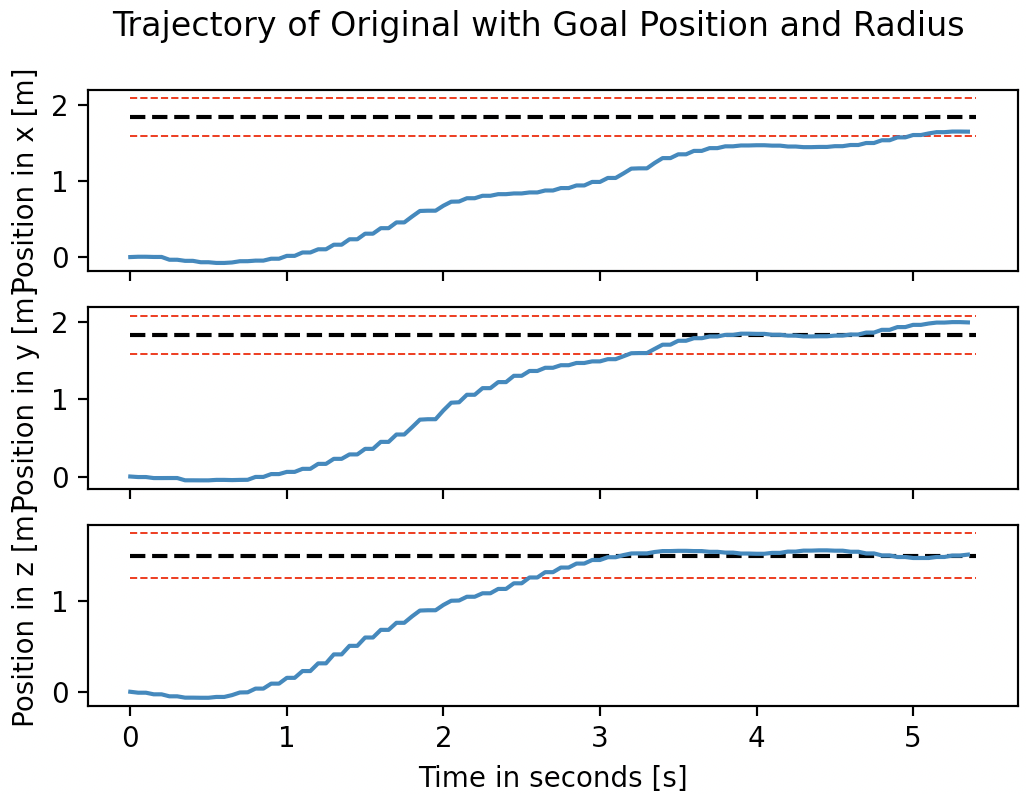
\includegraphics[width=\textwidth]{figures/5_/Testing/ddpg_test_original2.png}
         \caption{The trajectory of the quadrotor with the Original model compared to the goal position, decomposed in $x$, $y$, $z$.}
         \label{fig:testing_ddpgOriginal2}
     \end{subfigure} 
    \captionsetup{justification=centering}
    \caption{Test run no. 100 for the Modified and Original DDPG models.}
     \label{fig:5_testing_DDPG}
\end{figure}
From Figures \ref{fig:testing_ddpgModified1} and \ref{fig:testing_ddpgOriginal1}, it is clear that the Modified model performs best, with the smallest cross-track error over the whole episode and matching the result given in Table \ref{table:5_DDPG_tests}. This result is further highlighted in subplots (c) and (d), where the Modified run is significantly outperforms the Original in the $x$-axis, with similar performance in $y$ and $z$. We see also that the quadrotor is within the goal region at about 3 seconds in the Modified model, while it takes about 5 seconds to reach the same goal region for the Original model. The reason that the episode does not terminate earlier for the Modified model, is probably due to its more aggressive response. In (a), the we can see that the spacing is marginally wider than that in (b), showing a greater speed. We can therefore guess that the overall speed $||\v_t|| > 0.3$, such that we do not satisfy our goal condition in \eqref{4_goal_condition}. In contrast, when the Original controller reaches the goal region, the episode terminates instantly, which tells us that a gentle approach is made towards the goal. 

Nonetheless, the higher $\v_t$ is not significant enough to cause such a difference in the average return. Instead, our guess is that the average return for the Modified model in \ref{table:5_DDPG_tests} is actually an error. To take a closer look at this, both models were checked to see which episodes did not result in a goal. Interestingly, episode 7 was disastrous for the Modified model, seen in the table below:
\begin{table}[H]
    \centering
    \begin{tabular}{||c||c|c||}
    \hline
    \multicolumn{3}{||c||}{Episode Data for Test Runs no. 7 and 51} \\
    \hline\hline
        Episode Total squared-error & 5799.8317 & 286.0620 \\ 
        Episode steps & 181 & 181  \\
        Episode RMSE & 0.4208 & 0.0934\\
        Episode Return & -88.259 & -8.367 \\
    \hline
    \end{tabular}
    \caption{Failed test runs no. 7 and 51 for the Modified DDPG model. Note the large episode RMSE and return, compared to that in Table \ref{table:5_DDPG_tests}.}
    \label{tab:5_DDPG_errorTestRun}
\end{table}
Test run no. 7 was a significant anomaly in the test data, even when compared to run 51. Therefore in my opinion, it is more insightful and beneficial to neglect these in the comparison. So, by taking into consideration only the test runs that resulted in a reaching the goal state, we obtain Table \ref{table:5_DDPG_adjustedtests}.
\begin{table}[hbt]
    \centering
    \begin{tabular}{||M{2cm}||M{2.5cm}|M{2.5cm}|M{2.5cm}||}
    \hline
    Model & Goal Rate & Average Return & Average RMSE \\\hline\hline
    NTNU     & 0      & -6.539     & 0.170 \\\hline
    Original & 100    & 0.183      & 0.037   \\\hline
    Modified & 100    & 0.267      & 0.025
     \\\hline
    \end{tabular}
    \caption{The adjusted test results for the DDPG models, where 4.}
    \label{table:5_DDPG_adjustedtests}
\end{table}
From this table, we see that the adjusted test results are now all in agreement with each other, and we obtain an average return which reflects the goal bonus of +1 much more clearly.


\subsubsection{Robustness Test with $\pm10\%$ Mass}
\label{sec:5_ddpg_robustnessTests}
The last result that we have is the robustness test results for when the quadrotor mass is altered by a factor 0.1. With our simulated RMF weighing 500g, this was an additional or removed 50g. For this test, only the Original and Modified models were tested. The results are shown in Table \ref{table:5_DDPG_robustnesstests}.
\begin{table}[hbt]
    \centering
    \begin{tabular}{||M{2.3cm}||M{2.5cm}|M{2.5cm}|M{2.5cm}||}
    \hline
    Model & Goal Rate & Average Return & Average RMSE \\\hline\hline
         \textbf{+10\% Mass} &           &            &          \\\hline
Original & 0      & -1.414     & 0.039    \\\hline
Modified & 7      & -1.019     & 0.025   \\\hline\hline
         \textbf{-10\% Mass} &           &            &          \\\hline
Original & 0      & -65.841    & 0.595    \\\hline
Modified & 0      & -63.652    & 0.318  \\\hline
    \end{tabular}
    \caption{The robustness test results for the DDPG models, averaged over 100 episodes.}
    \label{table:5_DDPG_robustnesstests}
\end{table}
\begin{figure}[H]
     \centering
     \begin{subfigure}[b]{0.51\textwidth}
         \centering
         \captionsetup{justification=centering}
         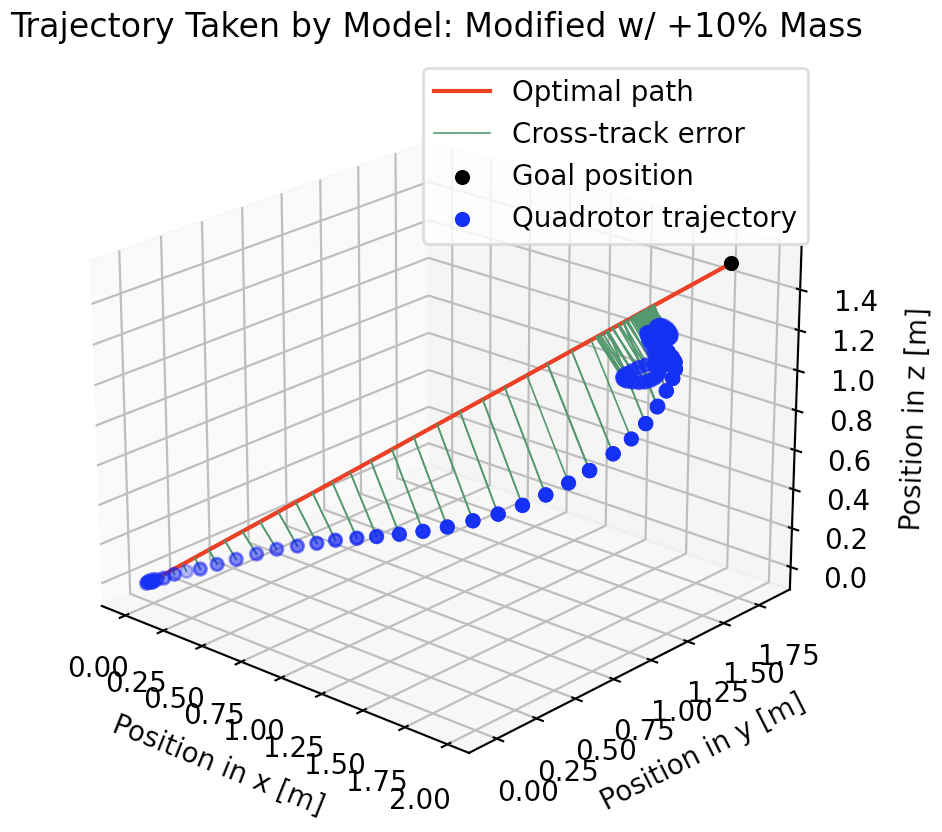
\includegraphics[width=\textwidth]{figures/5_/Testing/ddpg_test_robust+10-1.png}
         \caption{The trajectory of the quadrotor with +10\% mass, under guidance of Modified.}
         \label{fig:ddpg_test_robust+10-1}
     \end{subfigure} 
     \hfill 
     \begin{subfigure}[b]{0.48\textwidth}
         \centering
         \captionsetup{justification=centering}
         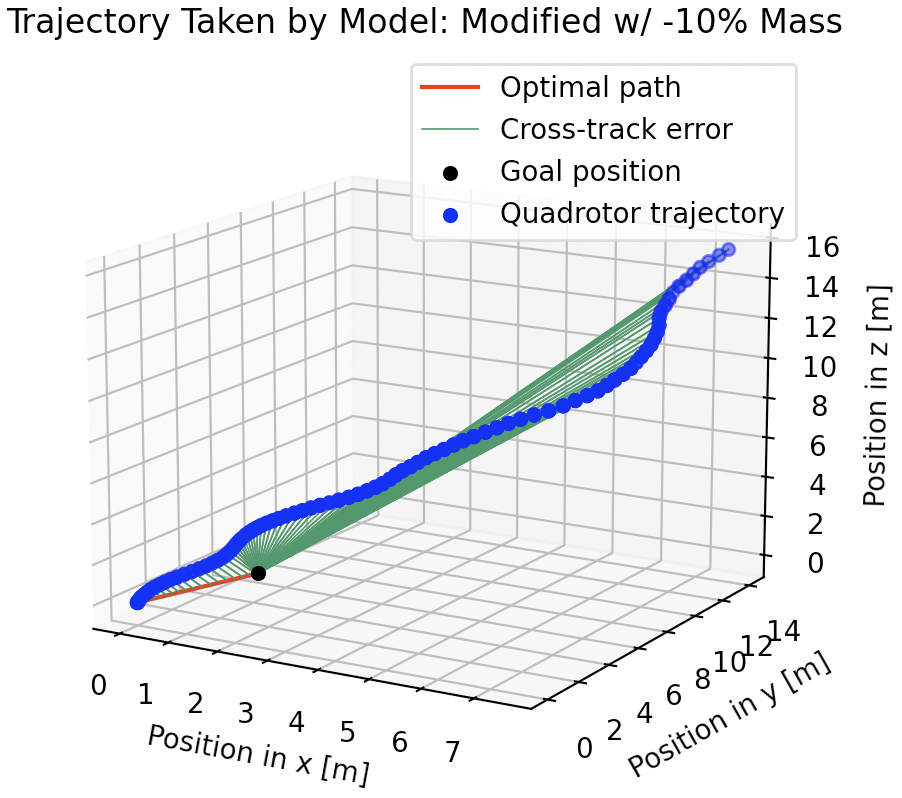
\includegraphics[width=\textwidth]{figures/5_/Testing/ddpg_test_robust-10-1.png}
         \caption{The trajectory of the quadrotor with -10\% mass, under guidance of Modified.}
         \label{fig:ddpg_test_robust-10-1}
     \end{subfigure} 
     \hfill \\[10mm]
     \begin{subfigure}[b]{0.49\textwidth}
         \centering
         \captionsetup{justification=centering}
         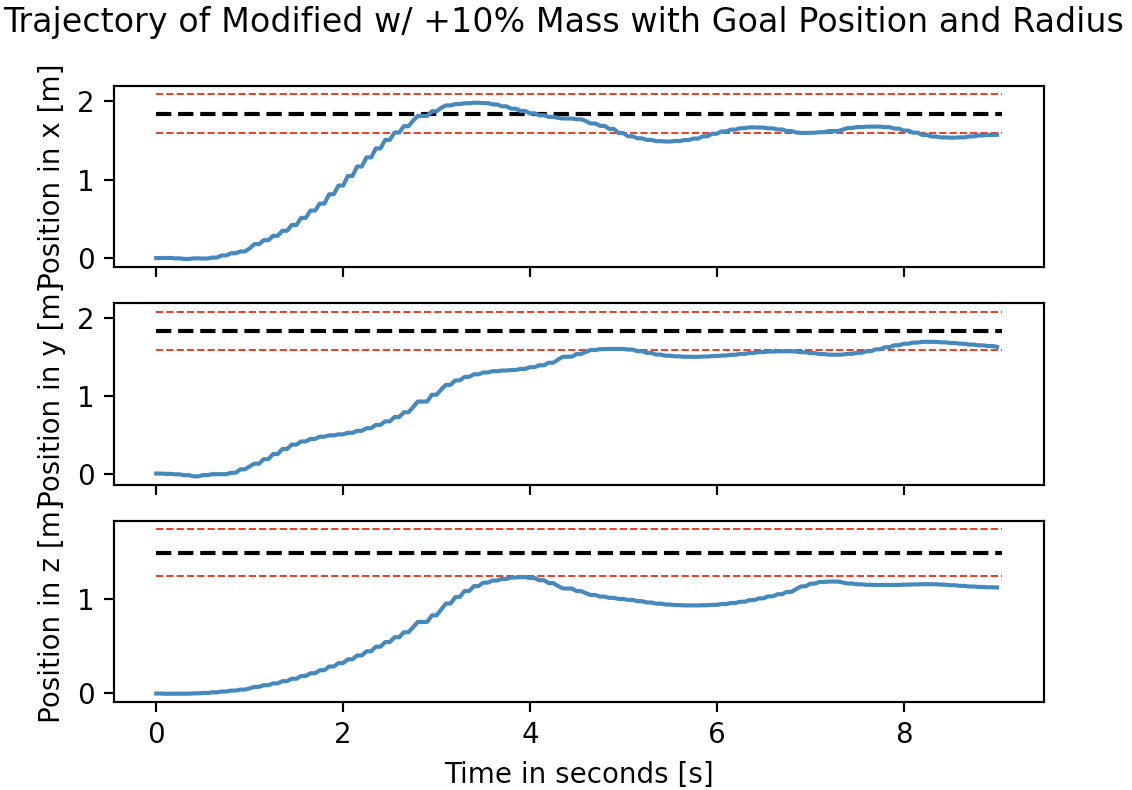
\includegraphics[width=\textwidth]{figures/5_/Testing/ddpg_test_robust+10-2.png}
         \caption{The trajectory of the quadrotor with +10\% mass, compared to the goal position, under guidance of the Modified model.}
         \label{fig:ddpg_test_robust+10-2}
     \end{subfigure} 
     \hfill 
     \begin{subfigure}[b]{0.49\textwidth}
         \centering
         \captionsetup{justification=centering}
         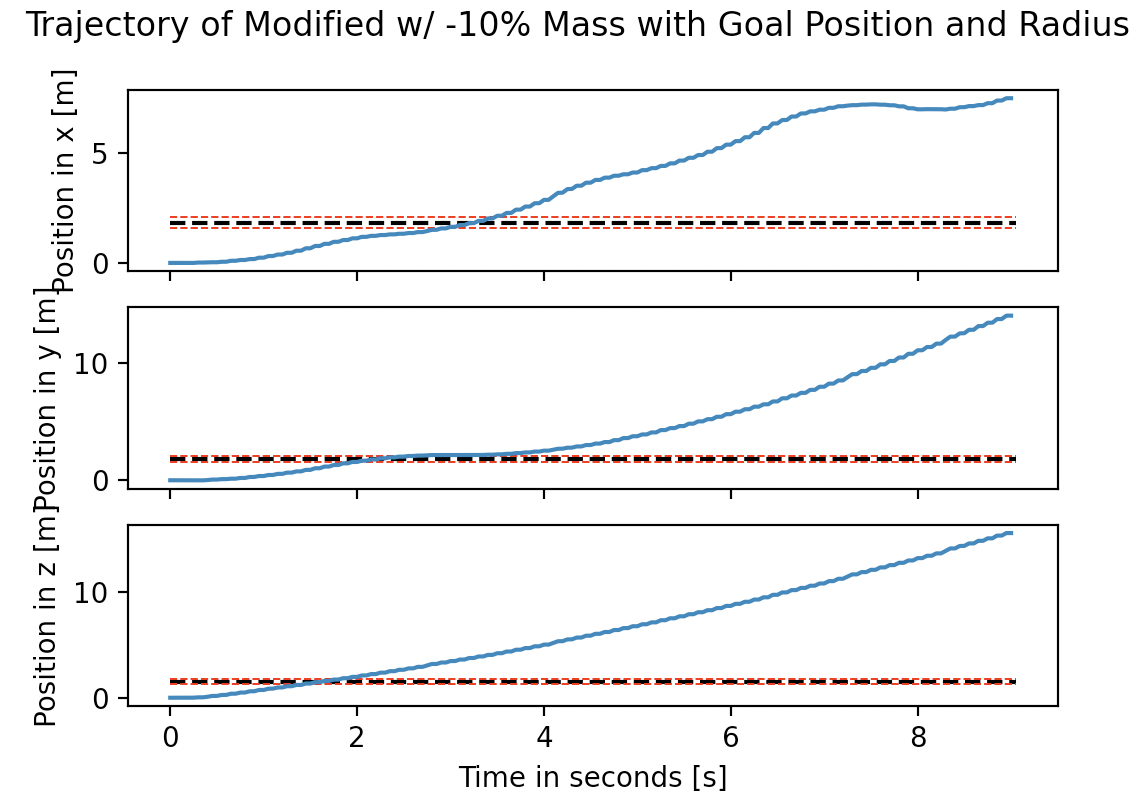
\includegraphics[width=\textwidth]{figures/5_/Testing/ddpg_test_robust-10-2.png}
         \caption{The trajectory of the quadrotor with -10\% mass, compared to the goal position, under guidance of the Modified model.}
         \label{fig:ddpg_test_robust-10-2}
     \end{subfigure} 
    \captionsetup{justification=centering}
    \caption{Test run no. 100 for the Modified and Original DDPG models.}
     \label{fig:ddpg_test_robust}
\end{figure}
From these results, we see that the performance of our DDPG models fall dramatically, with only the Modified model seldom being able to reach the goal in the +10\% mass case. We can also see that the performances in the -10\% mass case is severely impacted, compared to the +10\% case. To see why, we can take a look at Figure \ref{fig:ddpg_test_robust}.
From this figure, we observe two very contrasting behaviours. In the +10\% mass case, the quadrotor does decently to stay on track, settling quite nicely along $x$ and $y$ but struggles to match the goal position along the $z$-axis. In the -10\% mass case, the quadrotor overshoots the goal position by a large margin, basically flying off into the distance and unable to stop. From this, we see that the values in Table \ref{table:5_DDPG_robustnesstests} make sense.
Some considerations and possible explanations for why this happens will be made in Section \ref{sec:6_behaviour_robustnessTest_pm10}.


\section{PPO}
\label{sec:5_PPO}

As mentioned in Section \ref{sec:4_Experiment}, we majority of results are focused around PPO. The list of models are presented in Table \ref{table:5_PPO_hyperparameters}.
\begin{table}[hbt]
    \centering
    \resizebox{\textwidth}{!}{%
    \begin{tabular}{||M{0.7cm}|M{1.6cm}||M{1.8cm}|M{1.8cm}|M{1.7cm}|M{1.4cm}|M{1.4cm}|M{1.4cm}||}
    \hline
    ID & Model & Trajectory, T & Learning rate $\alpha$ & N. opt. epochs, K & N. minibatches & Ent. coef. $c_2$ & VF coef. $c_1$ \\ \hline\hline
    1  & 4-44$\alpha$ & 4000  & 2e-04 & 4  & 4 & 0    & 0.5 \\ \hline
    2  & 4-44       & 4000  & 3e-04 & 4  & 4 & 0    & 0.5 \\ \hline
    3  & 4-44E      & 4000  & 3e-04 & 4  & 4 & 0.01 & 0.5 \\ \hline
    4  & 4-84EV     & 4000  & 3e-04 & 8  & 4 & 0.01 & 1   \\ \hline
    5  & 8-44       & 8000  & 3e-04 & 4  & 4 & 0    & 0.5 \\ \hline
    6  & 8-84EV     & 8000  & 3e-04 & 8  & 4 & 0.01 & 1   \\ \hline
    7  & 8-88EV     & 8000  & 3e-04 & 8  & 8 & 0.01 & 1   \\ \hline
    8 & 8-154       & 8000  & 3e-04 & 15 & 4 & 0    & 0.5 \\ \hline
    9 & 8-154E      & 8000  & 3e-04 & 15 & 4 & 0.01 & 0.5 \\ \hline
    10 & 8-154EV    & 8000  & 3e-04 & 15 & 4 & 0.01 & 1   \\ \hline
    11 & 8-158EV    & 8000  & 3e-04 & 15 & 8 & 0.01 & 1   \\ \hline
    12 & 16-154     & 16000 & 3e-04 & 15 & 4 & 0    & 0.5 \\ \hline
    \end{tabular}%
    }
    \caption{The different PPO models tested, along with their hyperparameters.}
    \label{table:5_PPO_hyperparameters}
\end{table}
The model names here simply refer to its hyperparameters, where for example model 4, ``4-84EV'', has a batch size of 4000, makes 8 optimisations per trajectory, consist of 4 minibatches per trajectory, has an entropy coefficient of 0.01, and value function coefficient of 1.0. If a model does not contain E or V, the entropy and value function coefficients have the values of 0 and 0.5, as in the original implementation in \cite{baselines}. Also, the clipping term $\epsilon$ was chosen to be 0.1.

The choice of models in Table \ref{table:5_PPO_hyperparameters} was made so to be able to make a comparison between hyperparameters. These hyperparameters are initially inspired from the appendix in \cite{PPO}, with some modifications. There are quite a few combinations that did not make the list as over 80 models were tested for this project, with many of them experimental. Though, as a discussion, two of them will be briefly introduced in Section \ref{subsec:6_possible_improvements}.

Furthermore, every model tested here is trained from the same initialisation point to illustrate the effects of each hyperparameter more clearly. This was also decided because we managed to obtain a particularly impressive result from this initialisation point, which we wished to recreate.
Specifically, the initialisation point was a model 4-44 trained for 125 epochs, and the the impressive result was also a 4-44, which we will only look at at the end of this section.

\subsection{Training}
Training the models are done according to the description in Section \ref{sec:4_5_experimentalSetup}. The PPO models required significantly less time to train than its DDPG counterpart, though to reach questionable levels of performance. The epochs of best performance are varying for each of the models, handpicked from the training curves which we will see later.
The time taken to train each of the models to their peak are shown in Table \ref{table:5_PPO_trainingTime}. Note that every model is trained on top of a 4-44 model, trained to 125 epochs, which took 2 hours and 32 minutes.
\begin{table}[hbt]
    \centering
    \begin{tabular}{||M{1cm}|M{2cm}||M{2cm}|M{3cm}|M{3cm}||}
    \hline
    ID & Model & Peak Epoch & Training Time to Peak & Total Time \\ \hline\hline
    1  & 4-44$\alpha$ & 74 &   1h 25m &  3h 57m  \\\hline
    2  & 4-44       &   222 &  4h 16m &  6h 48m\\\hline
    3  & 4-44E      &   200 &  3h 51m &  6h 23m\\\hline
    4  & 4-84EV     &   114 &  2h 14m &  4h 46m\\\hline
    5  & 8-44       &   94 &   3h 36m &  6h 8m\\\hline
    6  & 8-84EV     &   155 &  6h 4m  &  8h 36m\\\hline
    7  & 8-88EV     &   131 &  5h 9m  &  7h 41m\\\hline
    8 & 8-154       &   104 &  3h 59m &  6h 31m\\\hline
    9 & 8-154E      &   110 &  4h 13m &  6h 45m\\\hline
    10 & 8-154EV    &   104 &  4m 1m  &  6m 33m\\\hline
    11 & 8-158EV    &   88 &   3h 26m &  5h 58m\\\hline
    12 & 16-154     &   113 &  8h 40m &  11h 12m\\\hline
    \end{tabular}
    \caption{The time used to train each of the PPO models presented. Since each model is initialised with a pre-trained 4-44 model, the total time compensates for the 2h 32m (125 epochs).}
     \label{table:5_PPO_trainingTime}
\end{table}
From the training times, we see quite a difference compared with the DDPG training times in Table \ref{table:5_PPO_trainingTime}, with the average training time being a third of that of DDPG.

When analysing the results for the training curves, we split the batch of models and only look at models relevant for each hyperparameter. Further, since the training plots are quite small and noisy, every data point is a smoothed with an exponential moving average with weight 0.9. We will also quickly see that the plots look very different compared to the ones for DDPG, though we will also come back to this later in the discussion. For now, the focus will be on the effect of the hyperparameters and the relative performance between the PPO models.

\subsubsection{Understanding The Actor-Critic Losses}
The actor and critic losses corresponds to the \textit{negative} clipped actor objective function $J_t^{CLIP}$ (in \cite{baselines}) and the MSE of the value function estimate and its bootstrapped target value -- the next-state reward and value estimate -- known as the prediction error $\overline{VE}$. These terms are found in Equation \eqref{3_5_objectiveFull}. 
Thus, the critic loss can be associated with PPO's ability to judge the value of its current state, similarly to in DDPG, where a high critic loss correlates to big discrepancies between value estimates in consecutive states, and a \textit{low critic loss} means that the value estimates in consecutive states are similar -- which happens if they are \textit{accurate}.

The actor objective function, $J_t^{CLIP}$, is positive if the advantage $\hat{A}_t$ is positive, which happens if the agent performs better than anticipated. The actor loss (the negative of  $J_t^{CLIP}$) is therefore negative if the agent performs better than anticipated and positive if the actor does worse than expected ($\hat{A}_t$ < 0). As for its magnitude, since $r_t(\bt)$ is clipped, the magnitude of the actor loss thus gives an estimate of how good or bad the actor did compared to its estimate, where then a \textit{large} positive actor loss means \textit{a lot} worse than expected. This follows from Equation \eqref{3_5_clippedObjective}, where $J_t^{CLIP}$ is proportional to $\hat{A}_t$, with $r_t(\theta) \in [1-\epsilon,\, 1+\epsilon]$ and $\epsilon = 0.1$. 


\subsubsection{Trajectory size}
So with interpretation of the plots clear, we can get underway with the results. The first hyperparameter to analyse is the length of the trajectory, $T$. For this, we compare models 4-44, 8-44, 8-154 and 16-154. 
\begin{figure}[hbt]
     \centering
     \begin{subfigure}[b]{0.32\textwidth}
         \centering
         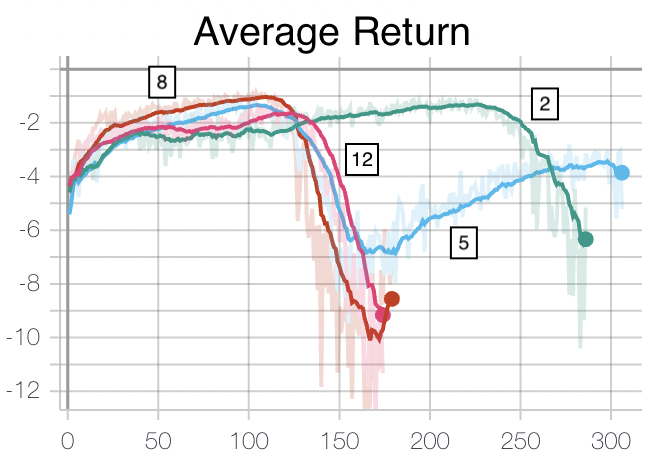
\includegraphics[width=\textwidth]{figures/5_/Training/ppo_trajectory_avgReturn.png}
         \caption{}
         \label{fig:5_training_ppo_trajectoryAvgReturn}
     \end{subfigure} 
     \hfill
     \begin{subfigure}[b]{0.32\textwidth}
         \centering
         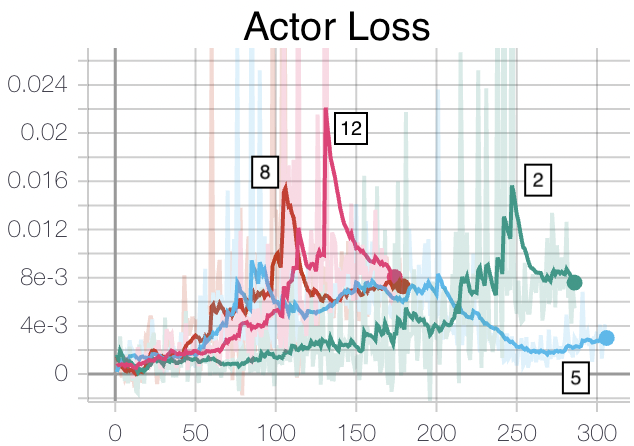
\includegraphics[width=\textwidth]{figures/5_/Training/ppo_trajectory_actorLoss.png}
         \caption{}
         \label{fig:5_training_ppo_trajectoryActorL}
     \end{subfigure}
     \hfill
     \begin{subfigure}[b]{0.32\textwidth}
         \centering
         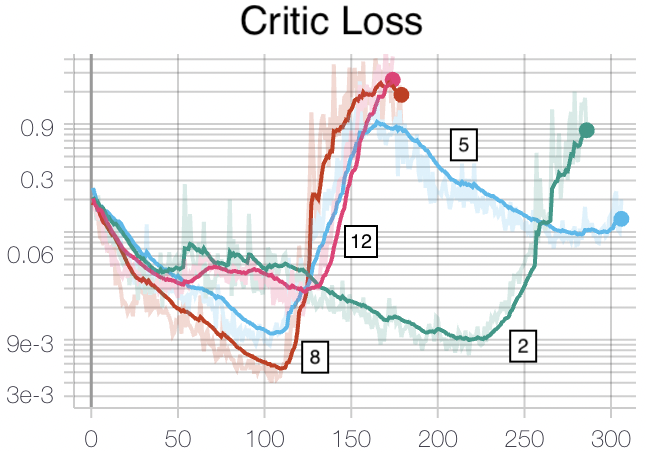
\includegraphics[width=\textwidth]{figures/5_/Training/ppo_trajectory_criticLoss.png}
         \caption{}
         \label{fig:5_training_ppo_trajectoryCriticL}
     \end{subfigure}
    \captionsetup{justification=centering}
    \caption{The effect of changing the length of the trajectory, $T$. There are two comparisons made, one between models 2: 4-44 and 5: 8-44, and the other between 8: 8-154 and 12: 16-154.}
     \label{fig:5_training_ppo_trajectory}
\end{figure}
From \cref{fig:5_training_ppo_trajectoryAvgReturn}, the effect of the trajectory length is varying. For models 2 and 5, we see that increasing the batch size from 4000 to 8000 does leads to faster training in terms of number of epochs, with both models reaching roughly the same average return at epochs 222 and 94. However, the ``speed'' is actually quite misleading, since one epoch requires double the number of experiences, such that the training times are also roughly the same. This can be confirmed through the training times in Table \ref{table:5_PPO_trainingTime} for models 2 and 5. Next, when the number of optimisation epochs are set to 15, we see that increasing the batch size further to 16000 from 8000 reduces performance, both in terms of peak average return, but also time required to train. 

We also see a correlation between the average return and critic loss, such that the agent gets better at predicting its value estimates at the same time it performs better in the environment too. It is unclear if there is some cause-effect at play between the two, but it makes sense that they are correlated since an agent performing well should be good at understanding the values of states and an agent who understands values of states will make good decisions.

For the actor loss, we can first observe that they are all positive. This means that the agent consistently finds its actions worse than expected, despite the critic getting better at estimate values of states and the average return increasing. Further, we also see spikes for each model which then are directly related to the sudden drop in average return. This means that when the average return drops, this is surprising to the agent as well and yields a large negative advantage. As the rate of change of return stabilises, then the actor loss reduces. Strangely however, there is a build up of actor loss \textit{before} each peak, which suggests that the agent thinks that is its performing increasingly worse than expected, despite that we can clearly see the average return increasing. This will be further explored in Section \ref{sec:6_underperformance_divergence_PPO}.

\subsubsection{Learning rate}
The next hyperparameter of interest is the learning rate, which has strong ties theoretical ties to the length of the trajectory (batch size) \cite{batchsizeInvariance,dontdecayLRIncreaseBatch,ImageNet1Hour}. The models compared are 4-44$\alpha$ and 4-44. 
\begin{figure}[hbt]
     \centering
     \begin{subfigure}[b]{0.32\textwidth}
         \centering
         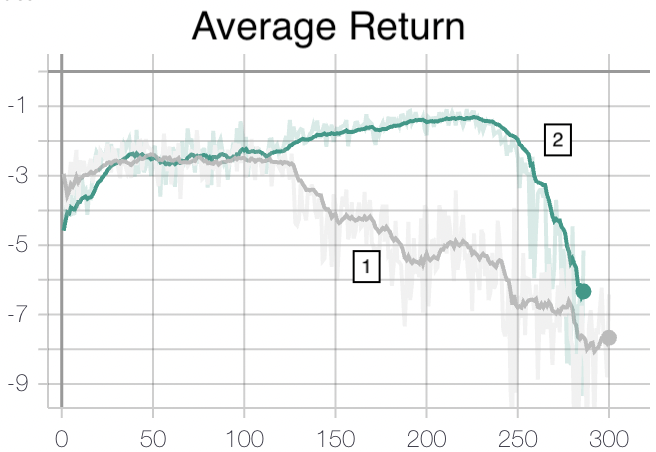
\includegraphics[width=\textwidth]{figures/5_/Training/ppo_learningRateAvgReturn.png}
         \caption{}
         \label{fig:5_training_ppo_learningRateAvgReturn}
     \end{subfigure} 
     \hfill
     \begin{subfigure}[b]{0.32\textwidth}
         \centering
         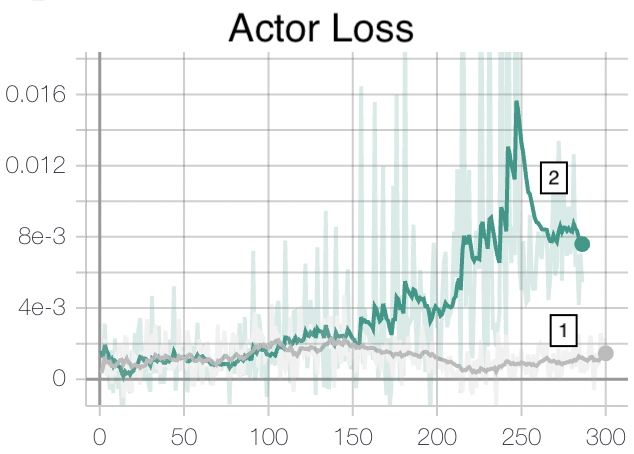
\includegraphics[width=\textwidth]{figures/5_/Training/ppo_learningRateActorL.png}
         \caption{}
         \label{fig:5_training_ppo_learningRateActorL}
     \end{subfigure}
     \hfill
     \begin{subfigure}[b]{0.32\textwidth}
         \centering
         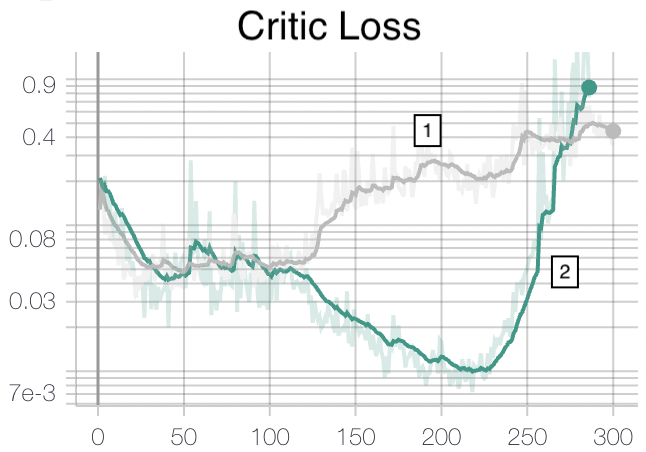
\includegraphics[width=\textwidth]{figures/5_/Training/ppo_learningRateCriticL.png}
         \caption{}
         \label{fig:5_training_ppo_learningRateCriticL}
     \end{subfigure}
    \captionsetup{justification=centering}
    \caption{The effect of changing the learning rate $\alpha$, seen through the comparison of models 1: 4-44$\alpha$ and 2: 4-44.}
     \label{fig:5_training_ppo_learningRate}
\end{figure}
From Figure \ref{fig:5_training_ppo_learningRate}, we see that reducing the learning rate from 3e-4 to 2e-4 leads to a lower performance on average, with no clear indication that model \one will improve beyond model 4-44, apart for when \two diverges. Interestingly, the actor loss is quite low with very minimal variance in consecutive epochs. This means that the agent does perform ``as expected'', though what this expectation is is a bit unclear given the high critic loss. This result is an example that reducing the learning rate in our implementation was not beneficial to performance, and so is the only comparison shown.


\subsubsection{Entropy Coefficient}
The entropy coefficient, in theory, should be related to the degree of exploration in seen in the agent. For on-policy methods, this is well-received and we hope to see the agents finding a better behaviour than in the previous plots. For this hyperparameter, we will comparing models, 4-44, 4-44E, 8-154 and 8-154E.
\begin{figure}[hbt]
     \centering
     \begin{subfigure}[b]{0.32\textwidth}
         \centering
         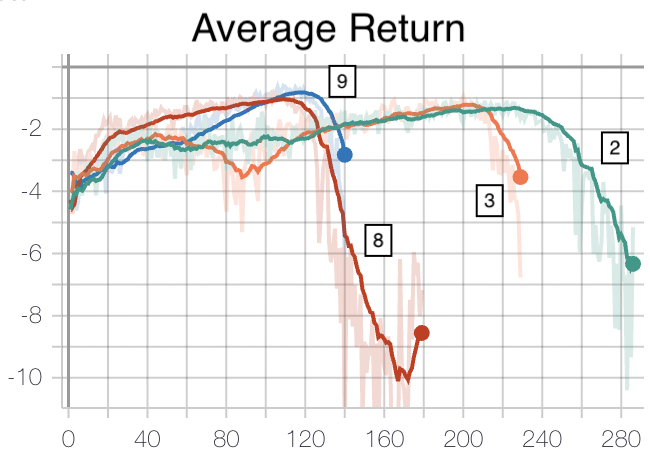
\includegraphics[width=\textwidth]{figures/5_/Training/ppo_entcoefAvgReturn.png}
         \caption{}
         \label{fig:5_training_ppo_entcoefAvgReturn}
     \end{subfigure} 
     \hfill
     \begin{subfigure}[b]{0.32\textwidth}
         \centering
         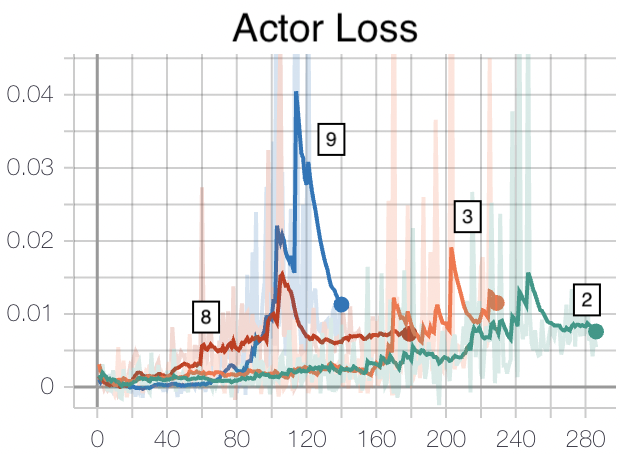
\includegraphics[width=\textwidth]{figures/5_/Training/ppo_entcoefActorL.png}
         \caption{}
         \label{fig:5_training_ppo_entcoefActorL}
     \end{subfigure}
     \hfill
     \begin{subfigure}[b]{0.32\textwidth}
         \centering
         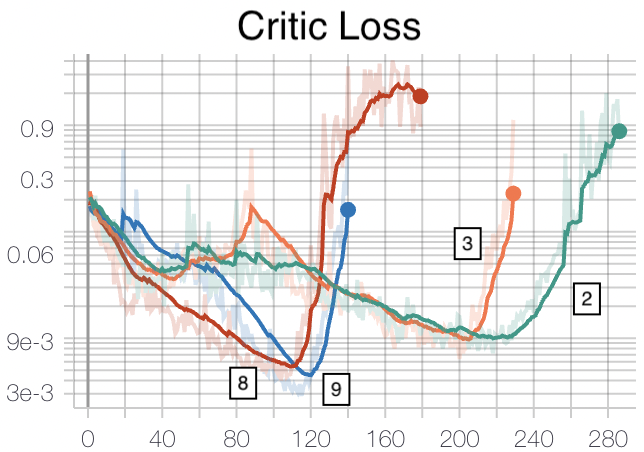
\includegraphics[width=\textwidth]{figures/5_/Training/ppo_entcoefCriticL.png}
         \caption{}
         \label{fig:5_training_ppo_entcoefCriticL}
     \end{subfigure}
    \captionsetup{justification=centering}
    \caption{The effect of changing the entropy term coefficient, $c_2$. There are two comparisons made, between models 2: 4-44 and 3: 4-44E, and between 8: 8-154 and 9: 8-154E.}
     \label{fig:5_training_ppo_entcoef}
\end{figure}
From \cref{fig:5_training_ppo_entcoef}, we observe varying results. Adding entropy loss does not have a significant effect for the 4-44E model, but leads to a marginally better peak average return, seen in the 8-154E model. Without high expectations, this was a good indication that the entropy term was beneficial.

Another interesting result is that the actor losses for the entropy models peak higher than their no-entropy counterparts. Since the entropy loss term is independent of the clipped actor objective, and the average returns and critic losses are also quite similar, the reason for why this is is unclear.


\subsubsection{Value function Coefficient}
In this project, we increased the value function coefficient from 0.5 to 1.0. This does not directly change the value function loss, but determines its weight in the total loss. As a result, we should achieve larger updates to the critic with a higher coefficient. To see what happens, we will compare the models 8-154E and 8-154EV.
\begin{figure}[hbt]
     \centering
     \begin{subfigure}[b]{0.32\textwidth}
         \centering
         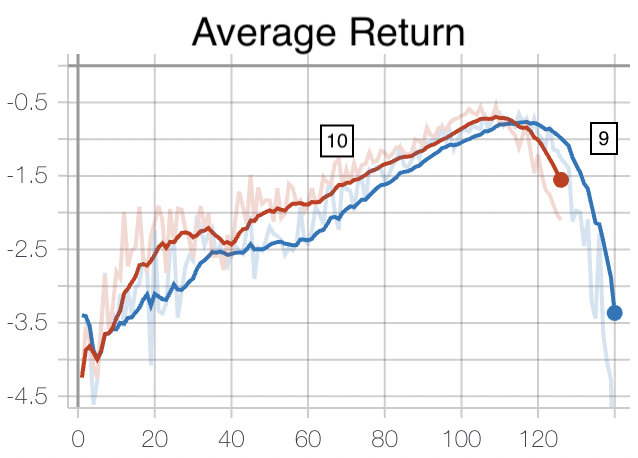
\includegraphics[width=\textwidth]{figures/5_/Training/ppo_vfcoeffAvgReturn.png}
         \caption{}
         \label{fig:5_training_ppo_vfcoeffAvgReturn}
     \end{subfigure} 
     \hfill
     \begin{subfigure}[b]{0.32\textwidth}
         \centering
         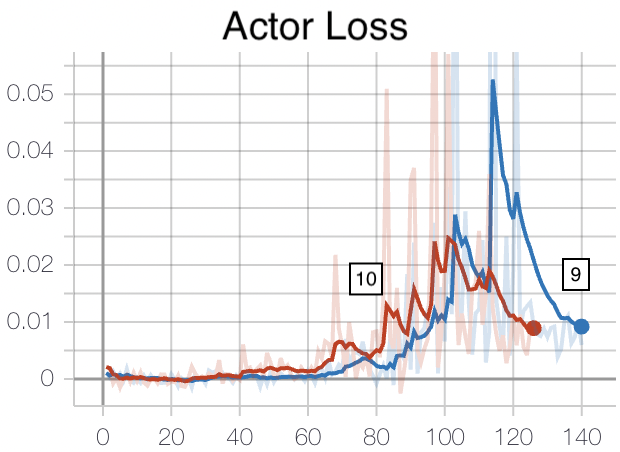
\includegraphics[width=\textwidth]{figures/5_/Training/ppo_vfcoeffActorL.png}
         \caption{}
         \label{fig:5_training_ppo_vfcoeffActorLoss}
     \end{subfigure}
     \hfill
     \begin{subfigure}[b]{0.32\textwidth}
         \centering
         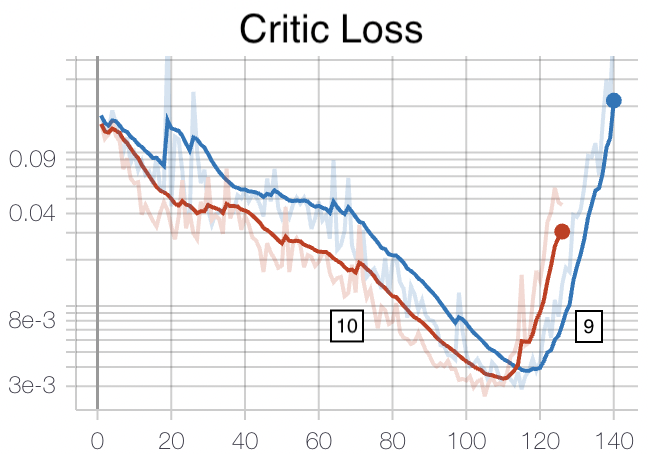
\includegraphics[width=\textwidth]{figures/5_/Training/ppo_vfcoeffCriticL.png}
         \caption{}
         \label{fig:5_training_ppo_vfcoeffCriticLoss}
     \end{subfigure}
    \captionsetup{justification=centering}
    \caption{The effect of changing the value function coefficient, $c_1$. This is a comparison between models 9: 8-154E and 10: 8-154EV.}
     \label{fig:5_training_ppo_vfcoeff}
\end{figure}
Based on Figure \ref{fig:5_training_ppo_vfcoeff}, we see that larger critic updates yields a slightly better performance overall. In \cref{fig:5_training_ppo_vfcoeffCriticLoss}, we observe that the critic loss in model \ten falls quicker than model \nine and matches our initial guess. Further, the relationship between the average return and the critic loss is highlighted clearly here, where our understanding that a low critic loss is beneficial to agent performance is true to a large extent.


\subsubsection{Number of optimisation epochs}
The number of optimisation epochs $K$, denotes the number of times we should update our weights based on the same trajectory. From this intuition, we expect that larger $K$ values should lead to faster learning, which could maybe lead to instability. 
\begin{figure}[hbt]
     \centering
     \begin{subfigure}[b]{0.32\textwidth}
         \centering
         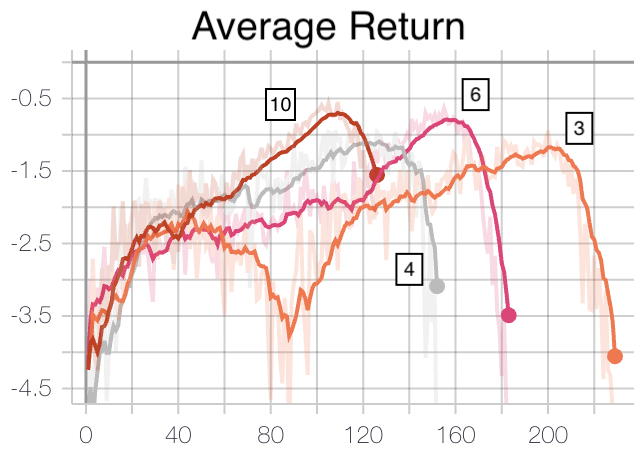
\includegraphics[width=\textwidth]{figures/5_/Training/ppo_noptepochsAvgReturn.png}
         \caption{}
         \label{fig:5_training_ppo_noptepochsAvgReturn}
     \end{subfigure} 
     \hfill
     \begin{subfigure}[b]{0.32\textwidth}
         \centering
         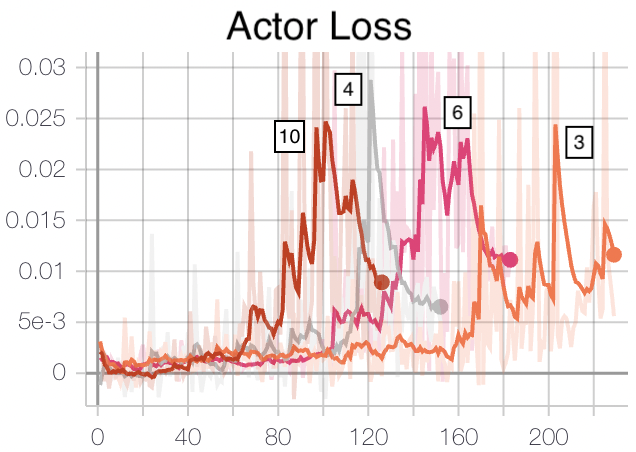
\includegraphics[width=\textwidth]{figures/5_/Training/ppo_noptepochsActorL.png}
         \caption{}
         \label{fig:5_training_ppo_noptepochsActorL}
     \end{subfigure}
     \hfill
     \begin{subfigure}[b]{0.32\textwidth}
         \centering
         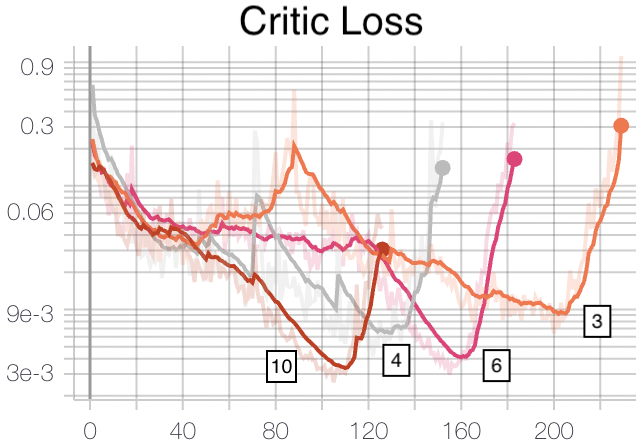
\includegraphics[width=\textwidth]{figures/5_/Training/ppo_noptepochsCriticL.png}
         \caption{}
         \label{fig:5_training_ppo_CriticL}
     \end{subfigure}
    \captionsetup{justification=centering}
    \caption{The effect of changing the number of optimisation epochs, $K$. Presented are two comparisons, between models 3: 4-44E and 4: 4-84EV, and 6: 8-84EV and 10: 8-154EV}
     \label{fig:5_training_ppo_noptepochs}
\end{figure}
\cref{fig:5_training_ppo_noptepochs} shows four models with similar shape, with models \ten and \six with highest average return, and \three and \four slightly below. From this, we see that there is no significant impact in the peak average return value when changing $K$, but we do observe that the \textit{training times are reduced significantly}. In that sense, our original expectation that instability occurs faster is also true. The actor and critic loss plots are very similar to the ones seen before and we can begin to see a trend in how the training curves are shaped for all models.


\subsubsection{Number of minibatches}
The number of minibatches indirectly controls the minibatch size, which is a hyperparameter often tuned in deep learning. From this, we know that small minibatches produce more noisy gradient updates compared to full-batch gradient updates. For this hyperparameter we will be comparing models 8-84EV, 8-88EV, 8-154EV and 8-158EV.
\begin{figure}[hbt]
     \centering
     \begin{subfigure}[b]{0.32\textwidth}
         \centering
         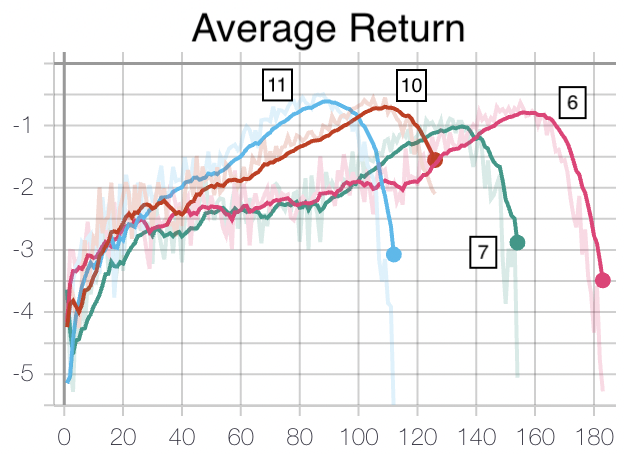
\includegraphics[width=\textwidth]{figures/5_/Training/ppo_nminibatchAvgReturn.png}
         \caption{}
         \label{fig:5_training_ppo_nminibatchAvgReturn}
     \end{subfigure} 
     \hfill
     \begin{subfigure}[b]{0.32\textwidth}
         \centering
         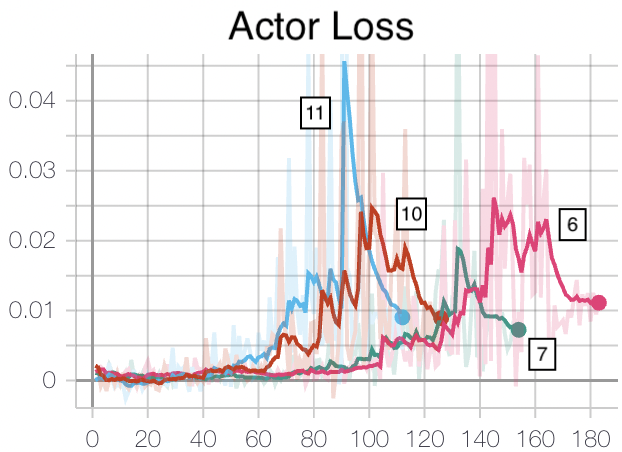
\includegraphics[width=\textwidth]{figures/5_/Training/ppo_nminibatchActorL.png}
         \caption{}
         \label{fig:5_training_ppo_nminibatchActorL}
     \end{subfigure}
     \hfill
     \begin{subfigure}[b]{0.32\textwidth}
         \centering
         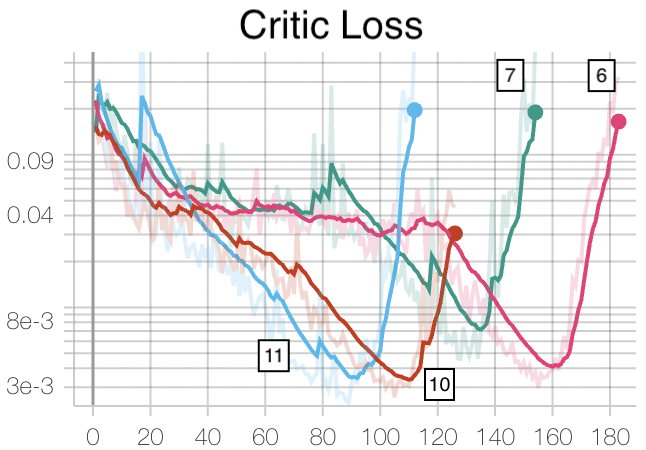
\includegraphics[width=\textwidth]{figures/5_/Training/ppo_nminibatchCriticL.png}
         \caption{}
         \label{fig:5_training_ppo_nminibatchCriticL}
     \end{subfigure}
    \captionsetup{justification=centering}
    \caption{The effect of changing the number of minibatches. There are two comparison for this, in models 6: 8-84EV, 7: 8-88EV, 10: 8-154EV, 11: 8-158EV.}
     \label{fig:5_training_ppo_nminibatch}
\end{figure}
In Figure \ref{fig:5_training_ppo_nminibatch}, we see that the training plots produced are not at all expected, given that the assumed effect of this hyperparameter was just more or less noisy updates. We observe that increasing the number of minibatches produces a similar response as that of the number of optimisation epochs, where the \textit{speed of learning} is significantly impacted. Apart from this, the effect on performance is varying, where doubling the number of minibatches in \seven leads to worse performance compared to 8-84EV, whereas \eleven has a slightly better performance than \ten. 

To explain this, a closer look was taken into the implementation of PPO in \cite{baselines}. From this we realised that the number of minibatches was also directly proportional to the number of gradient updates made. In other words, when the number of minibatches is doubled, so is the number of gradients calculated and applied to the networks, which is a bit obvious in hindsight. 
Based on this reasoning, it makes sense that doubling the number of minibatches results in roughly the same effect as doubling the number of optimisation epochs. 
Yet, exactly what happens is a bit unclear, since we expect the sum of losses per minibatch to be halved when the number of minibatches is doubled, so that despite more gradients applied, each gradient update is smaller. To guess why -- since we also clip the actor-objective -- taking many small gradient updates perhaps makes a larger overall update per epoch, compared to fewer larger updates when the number of minibatches is low, though this is not for certain.


\subsubsection{Best Models and the Optimal Model}
Now that we have seen the effect of different hyperparameters in training we look at some of the best models found. These are the models 8-84EV, 8-154E, 8-154EV and 8-158EV, shown in \cref{fig:5_training_ppo_bestModels}.
\begin{figure}[hbt]
     \centering
     \begin{subfigure}[b]{0.32\textwidth}
         \centering
         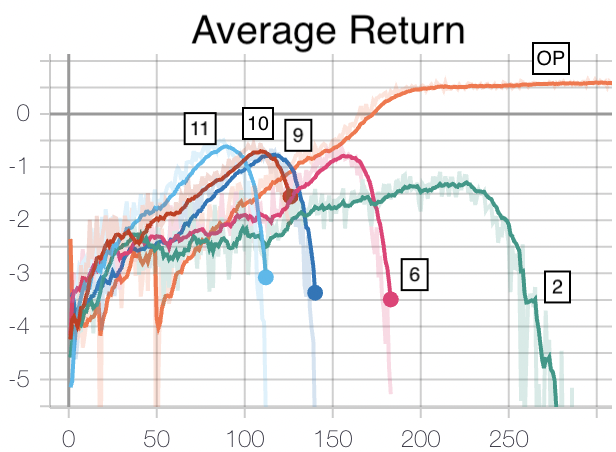
\includegraphics[width=\textwidth]{figures/5_/Training/ppo_bestmodelsAvgReturn.png}
         \caption{}
         \label{fig:5_training_ppo_bestModelsAvgReturn}
     \end{subfigure} 
     \hfill
     \begin{subfigure}[b]{0.32\textwidth}
         \centering
         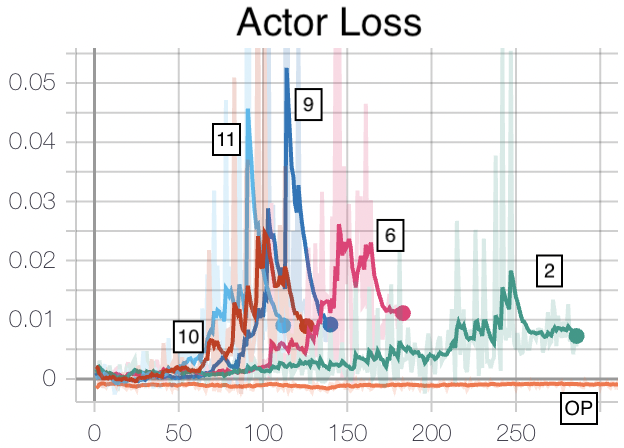
\includegraphics[width=\textwidth]{figures/5_/Training/ppo_bestmodelsActorL.png}
         \caption{}
         \label{fig:5_training_ppo_bestModelsActorL}
     \end{subfigure}
     \hfill
     \begin{subfigure}[b]{0.32\textwidth}
         \centering
         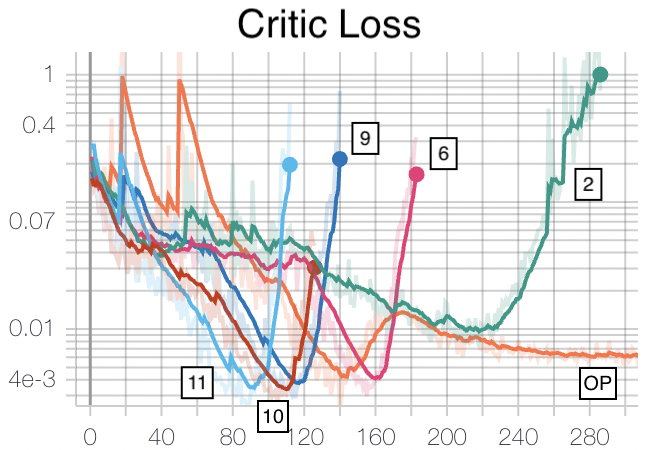
\includegraphics[width=\textwidth]{figures/5_/Training/ppo_bestmodelsCriticL.png}
         \caption{}
         \label{fig:5_training_ppo_bestModelsCriticL}
     \end{subfigure}
    \captionsetup{justification=centering}
    \caption{The training plots for the best models found for PPO. These are 6: 8-84EV, 9: 8-154E, 10: 8-154EV and 11: 8-158EV. Also included is our Optimal model, OP. Model 2: \two is included for reference.}
     \label{fig:5_training_ppo_bestModels}
\end{figure}
From this figure, we observe that the best average returns achieved are roughly the same, in between -0.5 and -0.9.
Looking very closely, there is a marginal difference, with model \eleven best, then 8-154EV, 8-154E, and
8-84EV. This is also the case for the lowest critic losses, though not so apparent in the smoothed \cref{fig:5_training_ppo_bestModelsCriticL}.
Unintuitively, \eleven also tops the ranking for the speed of training and took the shortest time to train to peak. 

We also present our optimally trained model, OP, which is of the same type as model 2 in \cref{fig:5_training_ppo_bestModels}, a 4-44. However, we see two very different training plots, where the OP model converges to an Optimal result with an average return of about 0.5, while Model 2 diverges.
We note that the OP model follows a similar training pattern as the other models though, with consistent improvement (seen until epoch 140) and a characteristic ``dip'' in the critic loss. However, as the other models then diverge after this dip, we see that the OP model instead is able to recover -- finding a ``good gradient descent path'' in the critic ``solution space'', and manages to keep improving its performance. This suggests that the ``dip'' in the critic loss and its corresponding peak in the average return could be understood as a \textit{local optimum} in the solution space that is simple to reach, while the \textit{global optimum} gradient descent path is much more difficult to find.

Another observation is that the actor loss for the OP model is always negative. This means that the agent always performed better than it expected, throughout its whole training period. This is very unique, since by pure randomness we would expect that at least at one point of its training should the agent do worse than it expected.


\subsubsection{Brief Summary}

All in all, we have seen that having a batch size of 8000 is beneficial to training in general, along with entropy and a higher value function coefficient. We observed that adding entropy loss for exploration was advantageous and slightly improved the peak average return, while the value function coefficient was a boost to reducing the critic loss, in turn improving training speed and slightly increased the peak average return.

To pair with this, one can choose to increase the number of optimisation epochs to either 8 or 15, while keeping the number of minibatches at 4 or increased to 8. These should then improve the training speed but not affect the peak average return attained.

Despite all our training efforts, the Optimal model does not follow this general guideline, but still managed to outperform all other models with a relatively simpler hyperparameter combination. This serves to remind us that hyperparameter tuning can only do so much in deep reinforcement leaning and the best models can be found unexpectedly with a bit of luck.


\subsection{Testing}
Now that we have seen the training results of our models we can begin to compare their performances in a standardised format to see if their training reflects their performance. In the Best Models section, it was briefly mentioned that the peaks in average returns for our models were possibly local optima. Thus, it will also be interesting to see what kind of behaviour this entails.

The test results are compiled into Table \ref{table:5_PPO_allTests}.
\begin{table}[hbt]
    \centering
    \begin{tabular}{||M{0.7cm}|M{1.6cm}||M{2.5cm}|M{2.5cm}|M{2.5cm}||}
    \hline
    ID & Model  & Goal rate & Average Return & Average RMSE   \\\hline\hline
    1	& 4-44$\alpha$ & 0 & -3.1027 &	0.1377 \\\hline
    2	& 4-44         & 0 & -2.3178 &	0.1000 \\\hline
    3	& 4-44E        & 0 & -2.1601 &	0.0767 \\\hline
    4	& 4-84EV       & 0 & -3.5790 &	0.0805 \\\hline
    5	& 8-44         & 0 & -1.9443 &	0.0528 \\\hline
    6	& 8-84EV       & 0 & -1.0316 &	0.0364 \\\hline
    7	& 8-88EV       & 0 & -2.5957 &	0.0685 \\\hline
    8	& 8-154        & 0 & -6.1768 &	0.1115 \\\hline
    9	& 8-154E       & 2 & -1.7125 &	0.0696 \\\hline
    10	& 8-154EV      & 3 & -3.0630 &	0.0660 \\\hline
    11	& 8-158EV      & 79 & -4.0786 &	0.0731 \\\hline
    12	& 16-154       & 0 & -2.6880 &	0.0693 \\\hline\hline
    OP & Optimal (4-44) & 100 &	0.4294 & 0.0181 \\\hline
    \end{tabular}
    \caption{The test results for all the PPO models. Each model was run 100 times on a constant waypoint task. Then, the goal rate, average return and average RMSE to the shortest path was recorded.}
     \label{table:5_PPO_allTests}
\end{table}
To do an analysis of how the different hyperparameters correlate to performance in tests, we will break down \cref{table:5_PPO_allTests} similarly to how the training results were presented.

\subsubsection{Trajectory size}
\begin{table}[hbt]
    \centering
    \begin{tabular}{||M{0.7cm}|M{1.6cm}||M{2.5cm}|M{2.5cm}|M{2.5cm}||}
    \hline
ID & Model  & Goal rate & Average Return & Average RMSE   \\\hline\hline
2  & 4-44   & 0 & -2.3178 & 0.1000 \\\hline
5  & 8-44   & 0 & -1.9443 & 0.0528 \\\hline
8  & 8-154  & 0 & -6.1768 & 0.1115 \\\hline
12 & 16-154 & 0 & -2.6880 & 0.0693
     \\\hline
    \end{tabular}
    \caption{The relevant PPO test results for comparing the length of the trajectory, $T$.}
    \label{table:5_PPO_test_trajectory}
\end{table}
For the length of the trajectory, it was found that there was no significant difference when training models 4-44 and 8-44, while model 8-154 was better than 16-154.
Looking at \cref{table:5_PPO_test_trajectory}, we see that there is a significant difference in test performances compared to training. First, we see that the average return and RMSE for model \five was better than 4-44, with model \five having almost half the RMSE on average.
Next, we see that \eight is much worse than 16-154. This is unexpected since the extent of the difference is very significant. Doing a check into the results for model 8-154, it was found that there were only four runs with a return less -6.18, but with an average return of less than $-63$. By removing these the average increases to -1.72, which explains a lot, but leads to another question of why these anomalies occur. Removing the 7 runs above the mean return for \five leads to an average of -1.75. Thus, its average return in \cref{table:5_PPO_test_trajectory} is very representative of the true return. This is also the case for model 4-44, with only one anomaly run (less than -2.45) with a return of -18.45, which leads to an adjusted average return of -2.15.


\subsubsection{Learning rate}
\begin{table}[hbt]
    \centering
    \begin{tabular}{||M{0.7cm}|M{1.6cm}||M{2.5cm}|M{2.5cm}|M{2.5cm}||}
    \hline
ID & Model  & Goal rate & Average Return & Average RMSE   \\\hline\hline
    1&	4-$\alpha$&	0&	-3.1027	&0.1377 \\\hline
    2&	4-44&	0&	-2.3178	&0.1000 \\\hline
    \end{tabular}
    \caption{The relevant PPO test results for comparing the learning rate, $\alpha$.}
    \label{table:5_PPO_test_learningRate}
\end{table}
Moving on the learning rate, we expect that model \two is
better 4-44$\alpha$.
From \cref{table:5_PPO_test_learningRate} we see that this expectation holds true, with model 4-44 having both a higher average return and lower RMSE than 4-44$\alpha$.

\subsubsection{Entropy Coefficient}
\begin{table}[hbt]
    \centering
    \begin{tabular}{||M{0.7cm}|M{1.6cm}||M{2.5cm}|M{2.5cm}|M{2.5cm}||}
    \hline
ID & Model  & Goal rate & Average Return & Average RMSE   \\\hline\hline
2 & 4-44   & 0 & -2.3178 & 0.1000 \\\hline
3 & 4-44E  & 0 & -2.1601 & 0.0767 \\\hline
8 & 8-154  & 0 & -6.1768 & 0.1115 \\\hline
9 & 8-154E & 2 & -1.7125 & 0.0696
     \\\hline
    \end{tabular}
    \caption{The relevant PPO test results for comparing the effect of the entropy coefficient, $c_2$.}
    \label{table:5_PPO_test_ent_coef}
\end{table}
As for the entropy coefficient, our expectation that entropy yields slightly better performances are also true, seen from \cref{table:5_PPO_test_ent_coef}.
This also includes the fact that the adjusted average return for model \eight is at roughly 1.72, while the average return for 8-154E is already lower than this, without adjustment.


\subsubsection{Value Function Coefficient}
\begin{table}[hbt]
    \centering
    \begin{tabular}{||M{0.7cm}|M{1.6cm}||M{2.5cm}|M{2.5cm}|M{2.5cm}||}
    \hline
ID & Model  & Goal rate & Average Return & Average RMSE   \\\hline\hline
9  & 8-154E  & 2 & -1.7125 & 0.0696 \\ \hline
10 & 8-154EV & 3 & -3.0630 & 0.0660
     \\\hline
    \end{tabular}
    \caption{The relevant PPO test results for comparing the effect of the value function coefficient, $c_1$.}
    \label{table:5_PPO_test_vf_coef}
\end{table}
For the value function coefficient, the average returns are not as expected, with model \ten having a lower return than 8-154E. However, we see that this is not true when considering both the goal rate and the average RMSE. Thus, a usual suspicion that there are anomalies in the test runs for \ten pulling its average down. Compensating for 11 runs with return less than -3, model \ten then has an average of -1.09. When removing the 21 runs with return less than -1.71 for 8-154E, the average return increases to -1.25. This discovery is then a strong result for the value function coefficient.

\subsubsection{Number of optimisation epochs}
\begin{table}[hbt]
    \centering
    \begin{tabular}{||M{0.7cm}|M{1.6cm}||M{2.5cm}|M{2.5cm}|M{2.5cm}||}
    \hline
ID & Model  & Goal rate & Average Return & Average RMSE   \\\hline\hline
3 & 4-44E  & 0 & -2.1601 & 0.0767 \\\hline
4  & 4-84EV  & 0 & -3.5790 & 0.0805 \\\hline
6  & 8-84EV  & 0 & -1.0316 & 0.0364 \\\hline
10 & 8-154EV & 3 & -3.0630 & 0.0660
     \\\hline
    \end{tabular}
    \caption{The relevant PPO test results for comparing the number of optimisation epochs, $K$.}
    \label{table:5_PPO_test_noptepochs}
\end{table}
In \cref{table:5_PPO_test_noptepochs}, we observe that the increasing the number of optimisation epochs results in significantly poorer performances overall. This does not fit our results from training, which suggests that the number of optimisation epochs should not affect performance in general, rather just the training time. 

However, we observe that while the average return is higher and RMSE lower, model \ten is able to reach the goal state while \six is not. Another consideration is that from the Trajectory comparison, we found that adjusting the returns for models \eight and \five resulted in average returns -1.72 and -1.75, which is in contrast to \cref{table:5_PPO_test_noptepochs}. However, having made the adjustment for model \ten already, we see that model model \six is still better compared to the adjusted values of model 8-154EV, which has an average return of 1.09 and RMSE of 0.04309. Thus, we see that model \six is in fact one of our best models.


\subsubsection{Number of minibatches}
\begin{table}[hbt]
    \centering
    \begin{tabular}{||M{0.7cm}|M{1.6cm}||M{2.5cm}|M{2.5cm}|M{2.5cm}||}
    \hline
ID & Model  & Goal rate & Average Return & Average RMSE   \\\hline\hline
6  & 8-84EV  & 0  & -1.0316 & 0.0364 \\\hline
7  & 8-88EV  & 0  & -2.5957 & 0.0685 \\\hline
10 & 8-154EV & 3  & -3.0630 & 0.0660 \\\hline
11 & 8-158EV & 79 & -4.0786 & 0.0731
     \\\hline
    \end{tabular}
    \caption{The relevant PPO test results for comparing the number of minibatches.}
    \label{table:5_PPO_test_nminibatches}
\end{table}
Our expectation from training is that number of minibatches should have the same effect as the number of optimisation epochs and therefore not affect performance. From \cref{table:5_PPO_test_nminibatches}, we see that when the number of minibatches is doubled, the average return decreases and the average RMSE increases, yet the likelihood of reaching goal increases.
Thus, the effect of the number of minibatches resembles the effect of the number of optimisation epochs in \cref{table:5_PPO_test_noptepochs} to a great extent.

To be sure, the results of \eleven were adjusted by removing its 8 below-average runs. This yielded a much higher average return of -0.1332 and RMSE of 0.0440. This result reflects the goal rate much better, but still does not explain why it has such significant anomaly runs. 
Nonetheless, we can still consider \eleven one of our best models.

\subsubsection{Best Models and the Optimal Model}
\begin{table}[hbt]
    \centering
    \resizebox{\textwidth}{!}{
    \begin{tabular}{||M{0.7cm}|M{1.8cm}||M{1.5cm}|M{2.5cm}|M{2cm}||M{2.5cm}|M{2.5cm}|M{1.5cm}||}
    \hline
ID & Model  & Goal rate & Average Return & Average RMSE & Avg. Return w/o outliers & Avg. RMSE w/o outliers & Num. outliers   \\\hline\hline
6  & 8-84EV  & 0   & -1.0316 & 0.0364 & -1.0316 & 0.0364 & 0 \\\hline
9  & 8-154E  & 2   & -1.7125 & 0.0696 & -1.4446 & 0.0657 & 1 \\\hline
10 & 8-154EV & 3   & -3.0630 & 0.0660 & -1.1990 & 0.0457 & 8 \\\hline
11 & 8-158EV & 79  & -4.0786 & 0.0731 & -0.1332 & 0.0440 & 8 \\\hline\hline
OP & Optimal (4-44) & 100 & 0.4294 & 0.0181 & 0.4294 & 0.0181 & 0
     \\\hline
    \end{tabular}}
    \caption{The best models and best hyperparameter combinations found for PPO. These are compared against our Optimal model, OP. Results that ignore episodes with an average return of less than -5 are also shown.}
    \label{table:5_PPO_test_bestModels}
\end{table}
The best models found for PPO are summarised in \cref{table:5_PPO_test_bestModels}.
We can start by observing that model 8-84EV is by far the most consistent model, achieving the highest average return and lowest RMSE, even after adjusting the results for the other models. In contrast, model \eleven is the most inconsistent model, having the most extreme outliers which negatively affects its otherwise good result.

Next, we observe that our Optimal model has a 100\% goal rate, achieving an average reward that reflects its training results very well.

\begin{figure}[H]
     \centering
     \begin{subfigure}[b]{0.48\textwidth}
         \centering
         \captionsetup{justification=centering}
         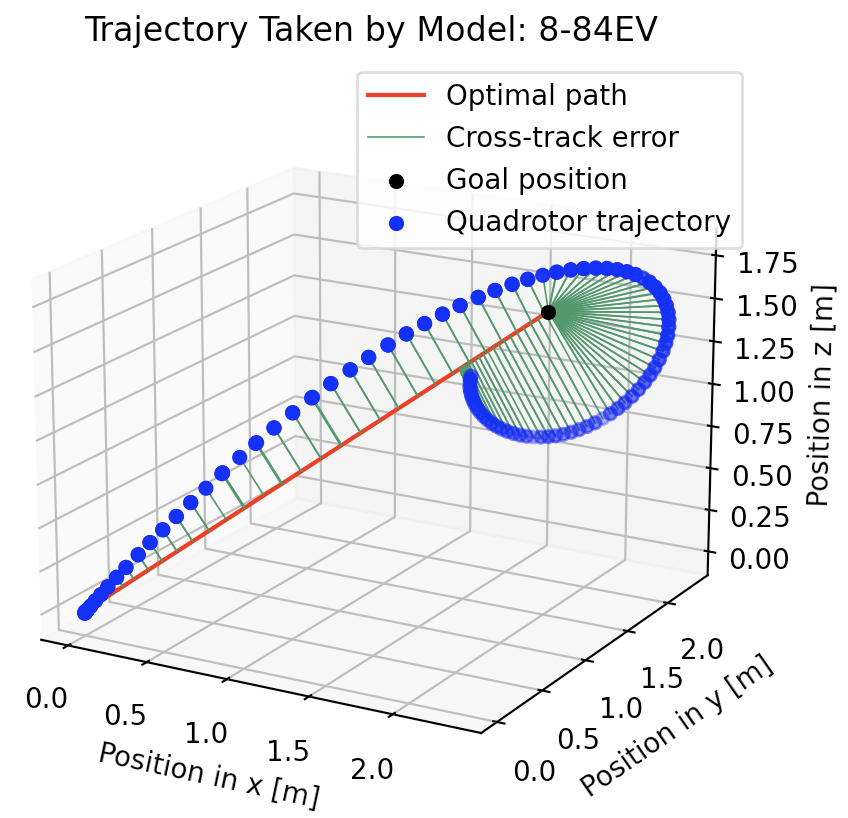
\includegraphics[width=\textwidth]{figures/5_/Testing/ppo_test_884EV1.png}
         \caption{Trajectory of 8-84EV.}
         \label{fig:testing_ppo884EV1}
     \end{subfigure} 
     \hfill 
    \begin{subfigure}[b]{0.49\textwidth}
         \centering
         \captionsetup{justification=centering}
         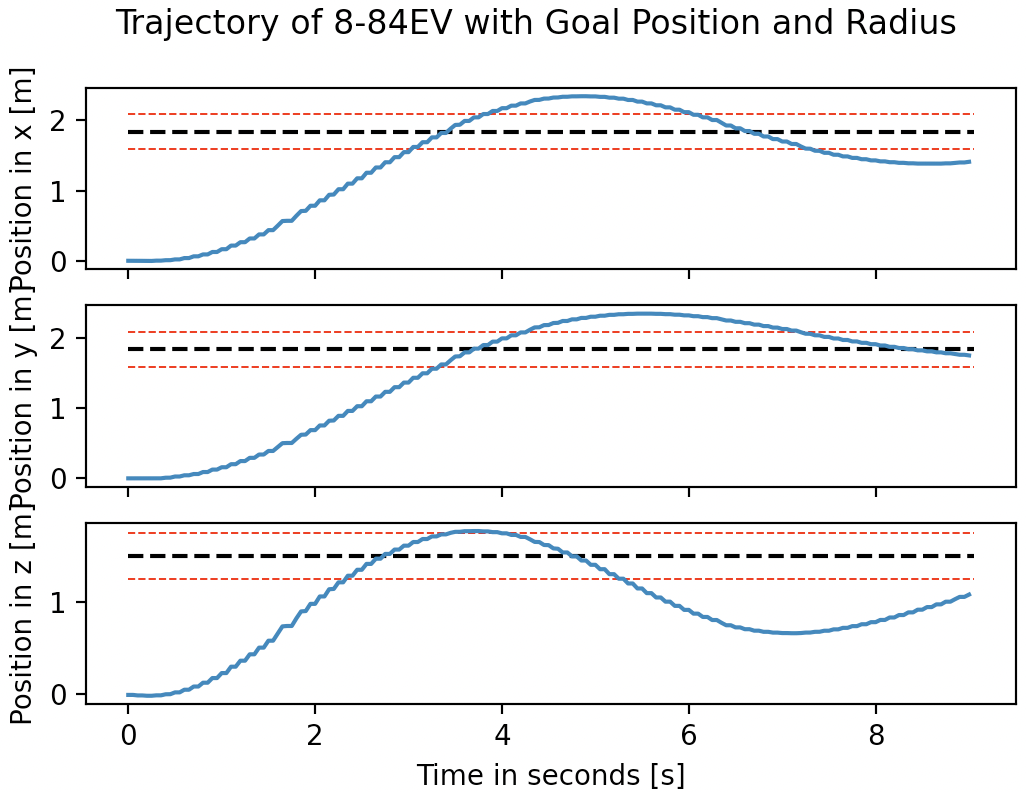
\includegraphics[width=\textwidth]{figures/5_/Testing/ppo_test_884EV2.png}
         \caption{Trajectory of 8-84EV, decomposed in $xyz$.}
         \label{fig:testing_ppo884EV2}
     \end{subfigure} 
     \hfill \\[1mm]
    \begin{subfigure}[b]{0.48\textwidth}
         \centering
         \captionsetup{justification=centering}
         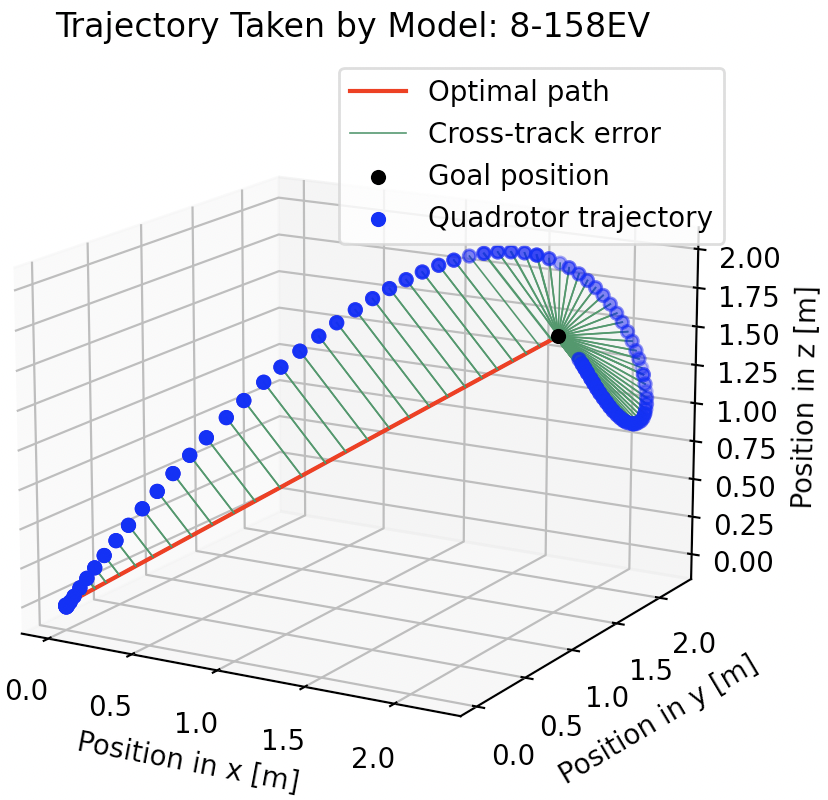
\includegraphics[width=\textwidth]{figures/5_/Testing/ppo_test_8158EV1.png}
         \caption{Trajectory of 8-158EV.}
         \label{fig:testing_ppo8158EV1}
     \end{subfigure} 
     \hfill 
     \begin{subfigure}[b]{0.49\textwidth}
         \centering
         \captionsetup{justification=centering}
         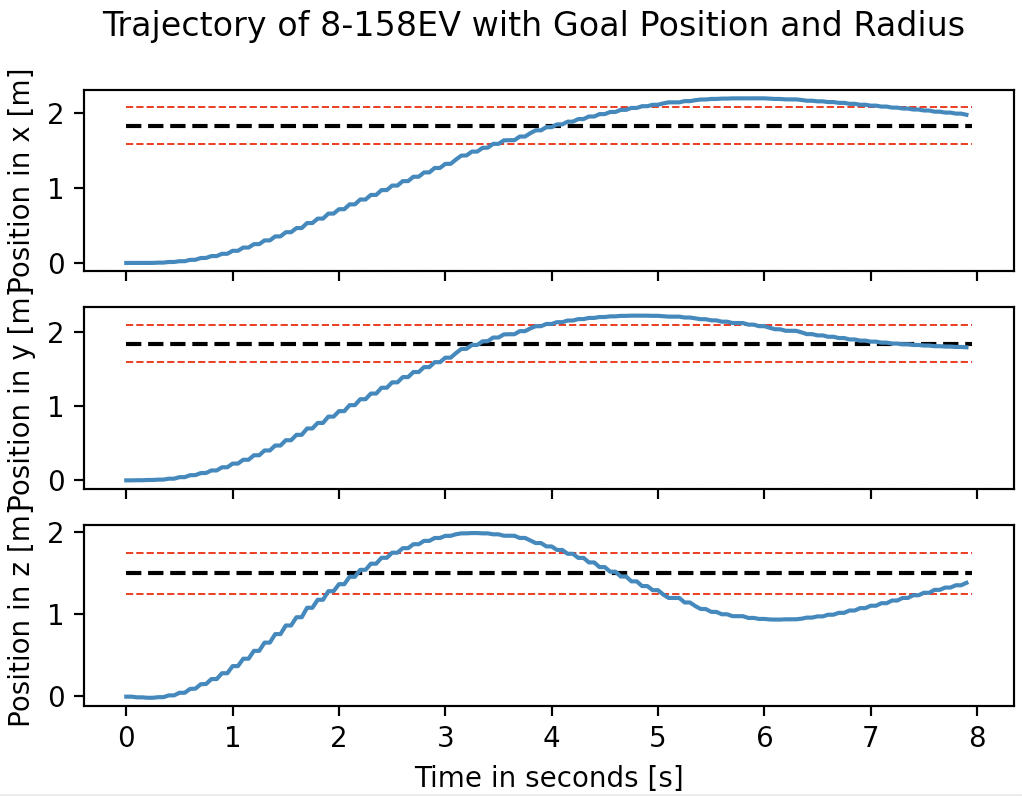
\includegraphics[width=\textwidth]{figures/5_/Testing/ppo_test_8158EV2.png}
         \caption{Trajectory of 8-158EV, decomposed in $xyz$.}
         \label{fig:testing_ppo8158EV2}
     \end{subfigure} 
     \hfill \\[1mm]
    \begin{subfigure}[b]{0.48\textwidth}
         \centering
         \captionsetup{justification=centering}
         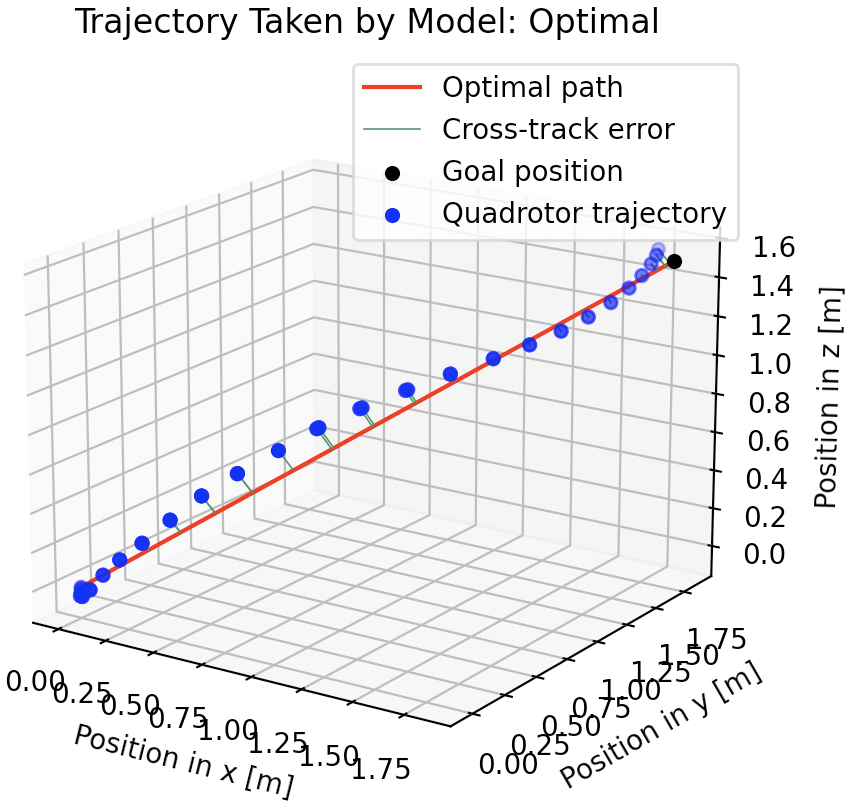
\includegraphics[width=\textwidth]{figures/5_/Testing/ppo_test_optimal1.png}
         \caption{Trajectory of Optimal.}
         \label{fig:testing_ppoOptimal1}
     \end{subfigure} 
     \hfill 
     \begin{subfigure}[b]{0.49\textwidth}
         \centering
         \captionsetup{justification=centering}
         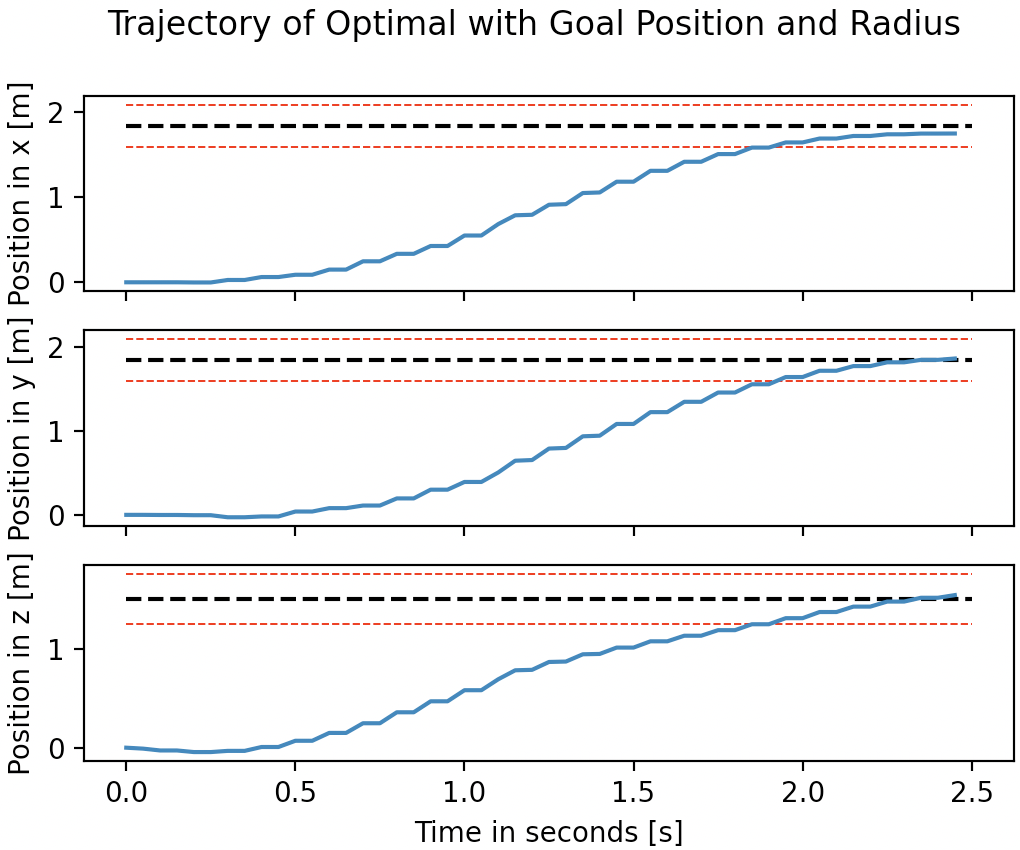
\includegraphics[width=\textwidth]{figures/5_/Testing/ppo_test_optimal2.png}
         \caption{Trajectory of Optimal, decomposed in $xyz$.}
         \label{fig:testing_ppoOptimal2}
     \end{subfigure}
    \captionsetup{justification=centering}
    \caption{Test run no. 100 for the 8-84EV, 8-158EV and Optimal PPO models.}
     \label{fig:5_testing_PPO}
\end{figure}
To look into detail of the behaviour of the PPO models, the trajectories for models 8-84EV, 8-158EV and Optimal are shown in \cref{fig:5_testing_PPO}.
Comparing the trajectories of the first two models we see that the 8-158EV model is just about able to reach the goal state at 8 seconds while the 8-84EV model is not. In addition, we see that both models overshoot the goal significantly along the $z$-axis, but is only slightly underdamped in $x$ and $y$. This makes sense from the reward function, where the $z$-term is weighted more than $x$ and $y$, such that the agent wishes to minimise this as fast as possible and perhaps judges overshoots as acceptable.

Moreover, the run no. 100 of model \six is very representative of the average run, having a return of -1.0372 and an RMSE of 0.03679. In contrast, run no. 100 of model \eleven is better than average, with a return of 0.1300 and an RMSE of 0.03861. Thus, both flights are very close in terms of RMSE, but model 8-158EV was much better at exploiting the reward function.

Lastly, for the Optimal model, we see that it reaches the goal with an optimal trajectory in just 2.5 seconds. We observe that there is no oscillatory behaviour, but instead a critically damped response, which shows that the agent has mastered the navigation task. 

\subsubsection{Robustness Test with $\pm10\%$ Mass}
\label{sec:5_ppo_robustnessTests}
Finally, to conclude the PPO tests we will assess the robustness of our best models. From experience in DDPG, it was decided that more time should be given to the models since the model performances were relatively lower. Thus, an extra 5 seconds was added to the timer such that the total time for each episode was 14 seconds. By running the same test with $\pm10\%$ mass and extra time, the results in \cref{table:5_PPO_robustnesstests} were achieved. 
\begin{table}[hbt]
    \centering
    \begin{tabular}{||M{2.3cm}||M{2.5cm}|M{2.5cm}|M{2.5cm}||}
    \hline
    Model & Goal Rate & Average Return & Average RMSE \\\hline\hline
         \textbf{+10\% Mass} &           &            &          \\\hline
8-84EV & 0     &  -2.8492   &  0.0750 \\\hline
8-158EV & 3      & -1.7590     & 0.0495    \\\hline
Optimal & 3      & -0.6705     & 0.0160   \\\hline\hline
         \textbf{-10\% Mass} &           &            &          \\\hline
8-84EV &   0     & -70.8971   &   0.3449  \\\hline
8-158EV &   0    &  -26.8076   &  0.2448 \\\hline
Optimal &   100    &  0.4636   & 0.0404  \\\hline
    \end{tabular}
    \caption{The robustness test results for the PPO models, averaged over 100 episodes. Note that 5 seconds extra was allocated to each episode.}
    \label{table:5_PPO_robustnesstests}
\end{table}
From this table, we see that that model \six struggles the most with these tests, with the being the most negatively impacted for both cases. Further, we can observe from the average RMSE that the +10\% mass case does not affect the trajectory of the quadrotor to a large degree, where models \ten and Optimal have roughly the same RMSEs as without any changes to mass. In the -10\% case, we see that the average RMSE for \ten is significantly worsened, yet the Optimal is not.  

As for the return and goal rate, model \ten struggles in both the +10\% case and -10\% case, with a significant drop in performance. We see that the Optimal model also struggles in the +10\% case but surprisingly manages a 100\% goal rate in the -10\% case.

Looking at Figures \ref{fig:5_testing_robust+10_PPO} and \ref{fig:5_testing_robust-10_PPO}, we observe a behaviour that is reflected in \cref{table:5_PPO_robustnesstests}. From these figures, it is also clear why there is such a low average return and high RMSE for models \six and \ten in the -10\% mass case. The main effect of added mass in the quadrotor results in the quadrotor is that the agent is unable to regulate its height to the goal position. As for its lateral positions, all models do relatively well, staying well within $\pm 1$m from the goal. In contrast, the -10\% mass case causes a drastic overshoot along all axes for models \six and 8-158EV, essentially amplifying the behaviour seen in \cref{fig:5_testing_PPO}. 
Through these examples, we can also confirm that model \ten outperforms model 8-84EV as it was able to maintain a trajectory closer to goal in both mass cases.

An interesting observation for both these models in the +10\% mass case is that both models display an oscillatory accelerate-brake behaviour in the $z$-position despite being nowhere near the goal. This is unexpected, as we should expect that the oscillation occurs around the goal position rather than under it. Thus, we will discuss this more in detail in Section \ref{sec:6_behaviour_robustnessTest_pm10}.

Lastly, for the Optimal model, we can see it was not able reach the goal in the +10\% mass case for the same reason as for the other models, because it was unable to regulate its height to the goal position. On the other hand, it is quite easily able to regulate its height in the -10\% mass case, with only a slight initial overshoot in the $z$-position. However, we can also see that values in \cref{table:5_PPO_robustnesstests} are quite unrepresentative of the Optimal model performance, since it portrays a much worse performance in the +10\% mass case compared to what is actually observed.
\begin{figure}[H]
     \centering
     \begin{subfigure}[b]{0.48\textwidth}
         \centering
         \captionsetup{justification=centering}
         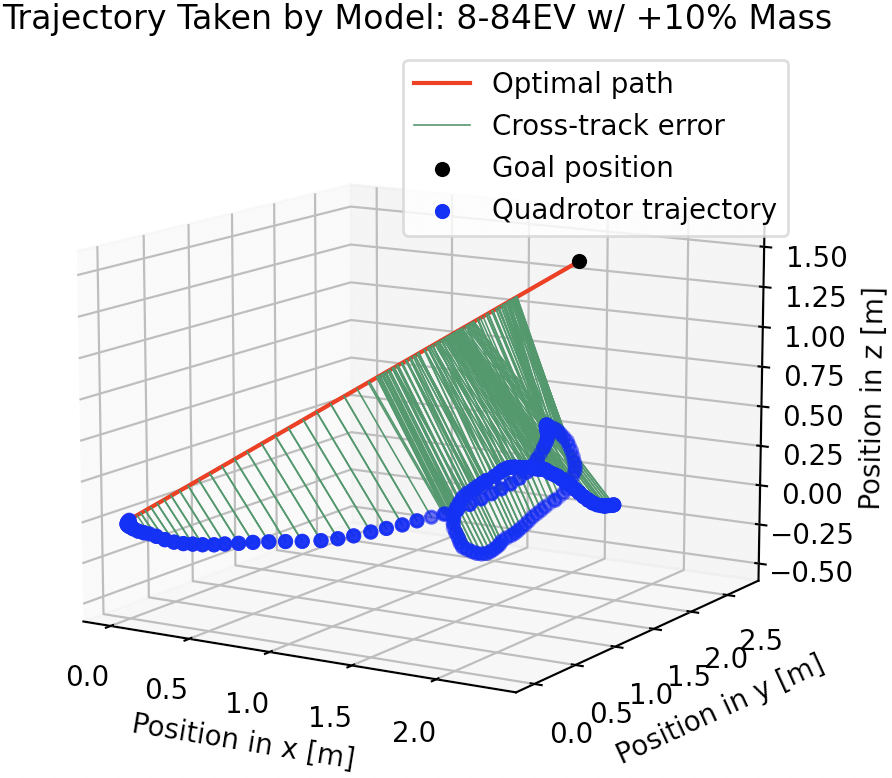
\includegraphics[width=\textwidth]{figures/5_/Testing/ppo_test_robust+10-884EV1.png}
         \caption{Trajectory of 8-84EV +10\% Mass.}
         \label{fig:testing_robust+10_ppo884EV1}
     \end{subfigure} 
     \hfill 
    \begin{subfigure}[b]{0.49\textwidth}
         \centering
         \captionsetup{justification=centering}
         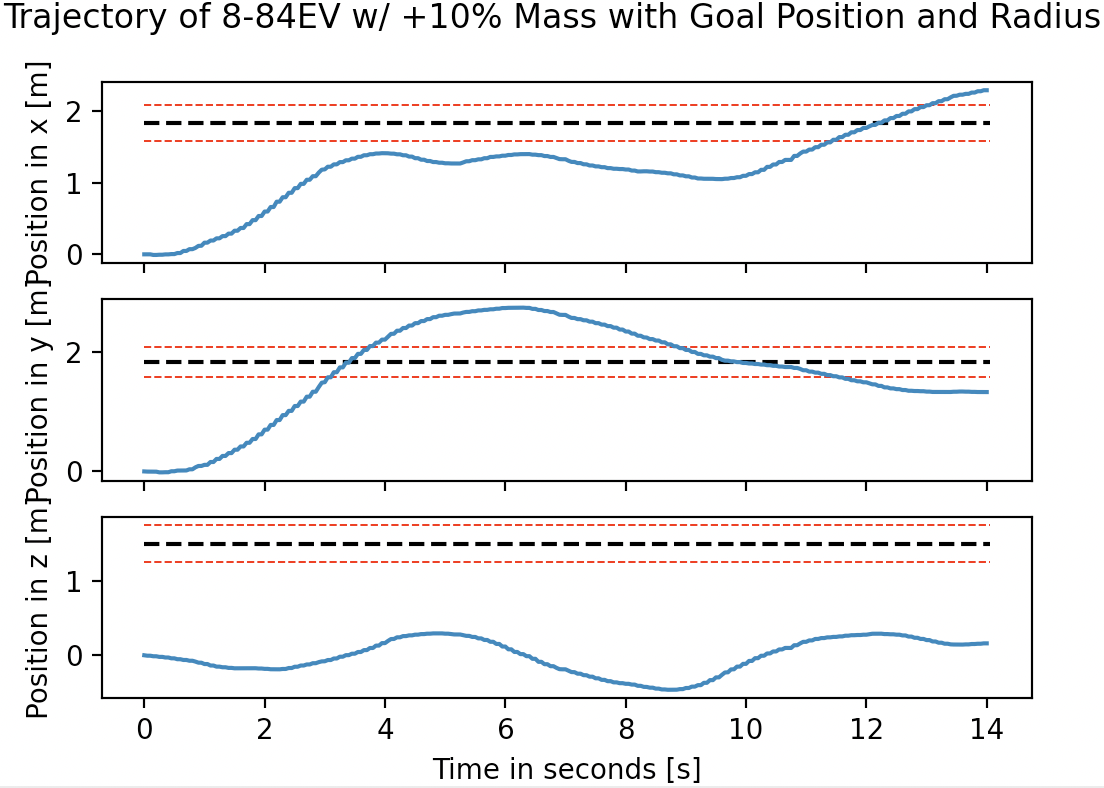
\includegraphics[width=\textwidth]{figures/5_/Testing/ppo_test_robust+10-884EV2.png}
         \caption{Trajectory of 8-84EV +10\% Mass, decomposed in $x$, $y$, $z$.}
         \label{fig:testing_robust+10_ppo884EV2}
     \end{subfigure} 
     \hfill \\[1mm]
    \begin{subfigure}[b]{0.48\textwidth}
         \centering
         \captionsetup{justification=centering}
         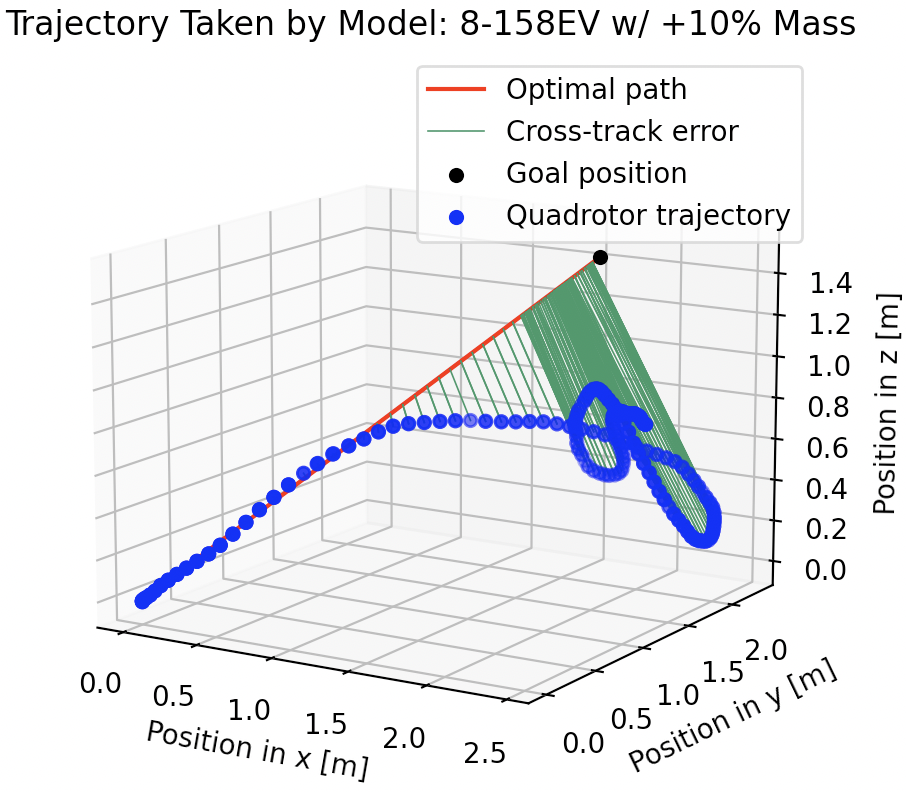
\includegraphics[width=\textwidth]{figures/5_/Testing/ppo_test_robust+10-8158EV1.png}
         \caption{Trajectory of 8-158EV +10\% Mass.}
         \label{fig:testing_robust+10_ppo8158EV1}
     \end{subfigure} 
     \hfill 
     \begin{subfigure}[b]{0.49\textwidth}
         \centering
         \captionsetup{justification=centering}
         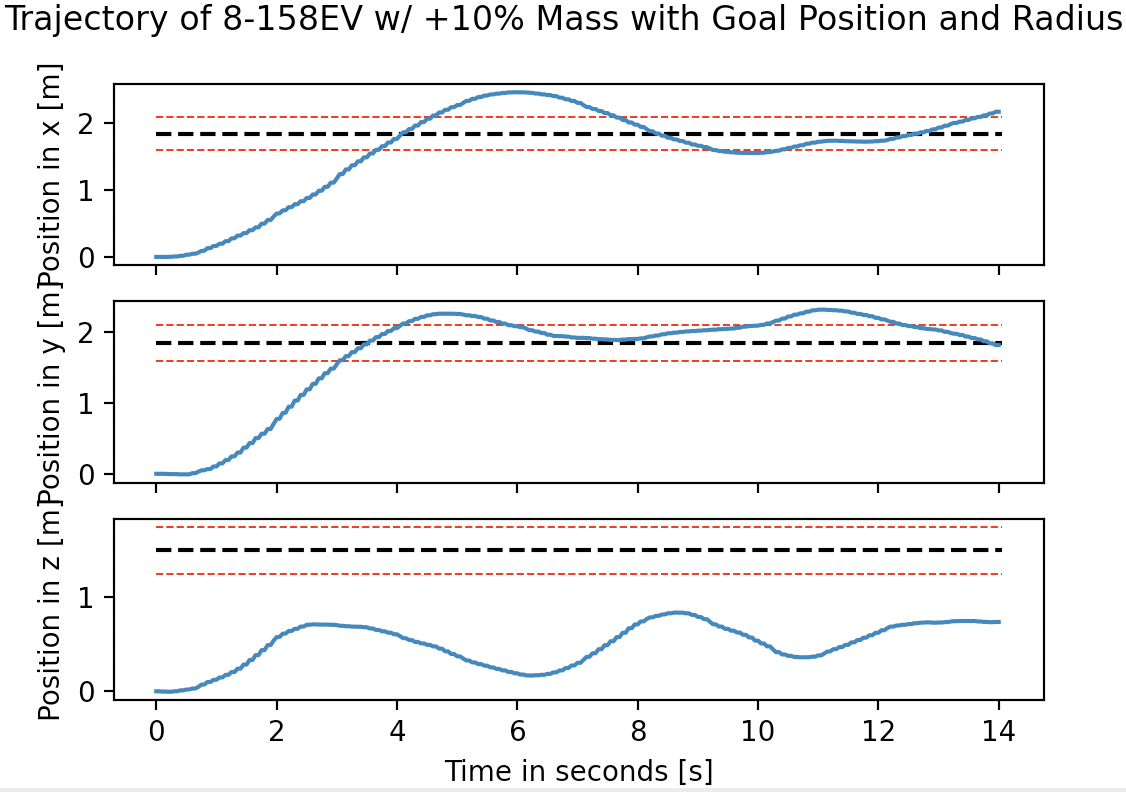
\includegraphics[width=\textwidth]{figures/5_/Testing/ppo_test_robust+10-8158EV2.png}
         \caption{Trajectory of 8-158EV +10\% Mass, decomposed in $x$, $y$, $z$.}
         \label{fig:testing_robust+10_ppo8158EV2}
     \end{subfigure} 
     \hfill \\[1mm]
    \begin{subfigure}[b]{0.48\textwidth}
         \centering
         \captionsetup{justification=centering}
         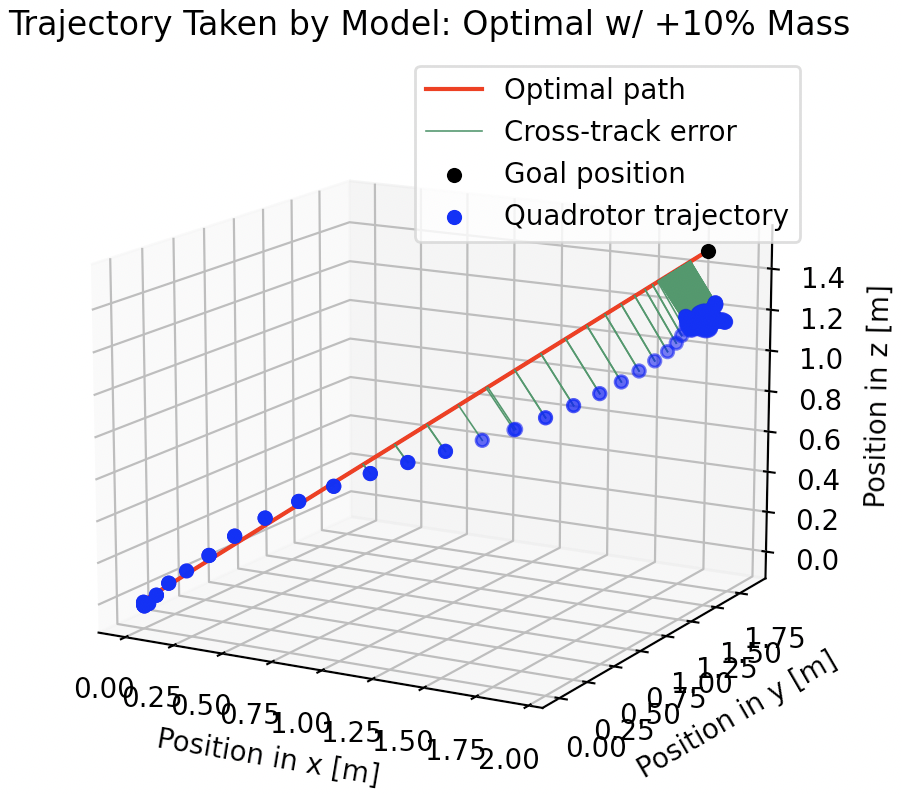
\includegraphics[width=\textwidth]{figures/5_/Testing/ppo_test_robust+10-Optimal1.png}
         \caption{Trajectory of Optimal +10\% Mass.}
         \label{fig:testing_robust+10_ppoOptimal1}
     \end{subfigure} 
     \hfill 
     \begin{subfigure}[b]{0.49\textwidth}
         \centering
         \captionsetup{justification=centering}
         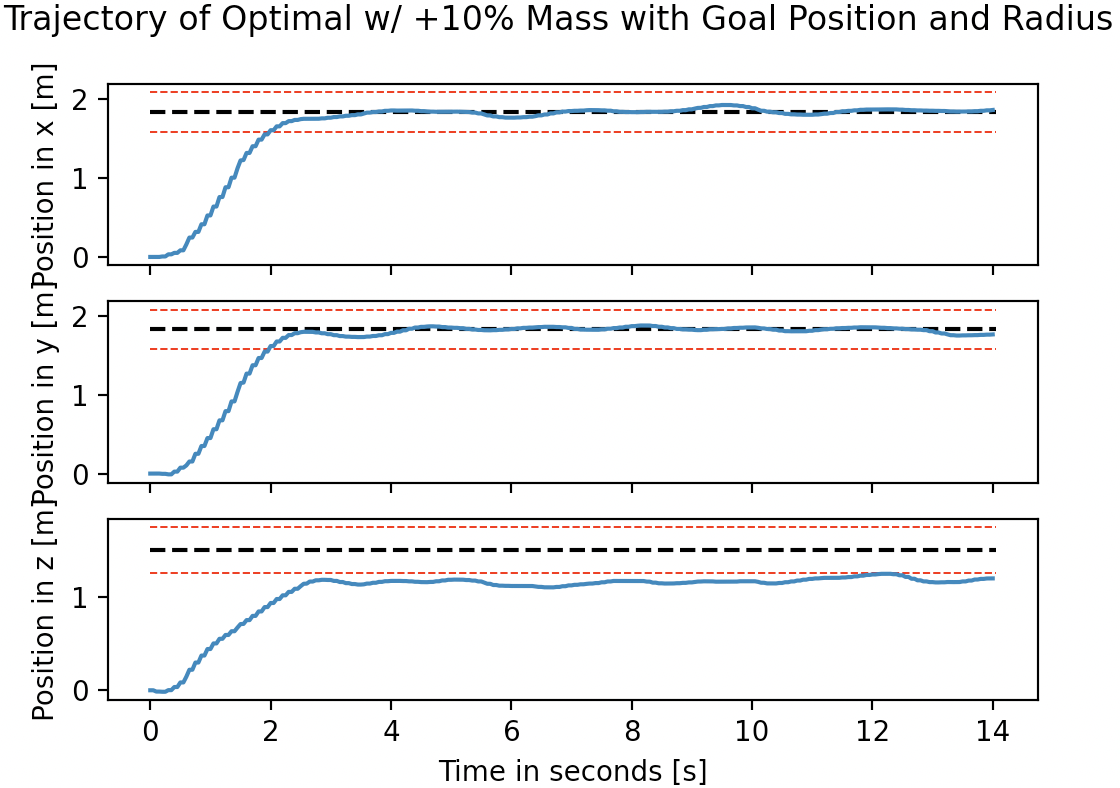
\includegraphics[width=\textwidth]{figures/5_/Testing/ppo_test_robust+10-Optimal2.png}
         \caption{Trajectory of Optimal +10\% Mass, decomposed in $x$, $y$, $z$.}
         \label{fig:testing_robust+10_ppoOptimal2}
     \end{subfigure}
    \captionsetup{justification=centering}
    \caption{Robustness test run no. 100 +10\% mass for 8-84EV, 8-158EV and Optimal PPO models.}
     \label{fig:5_testing_robust+10_PPO}
\end{figure}

\begin{figure}[H]
     \centering
     \begin{subfigure}[b]{0.48\textwidth}
         \centering
         \captionsetup{justification=centering}
         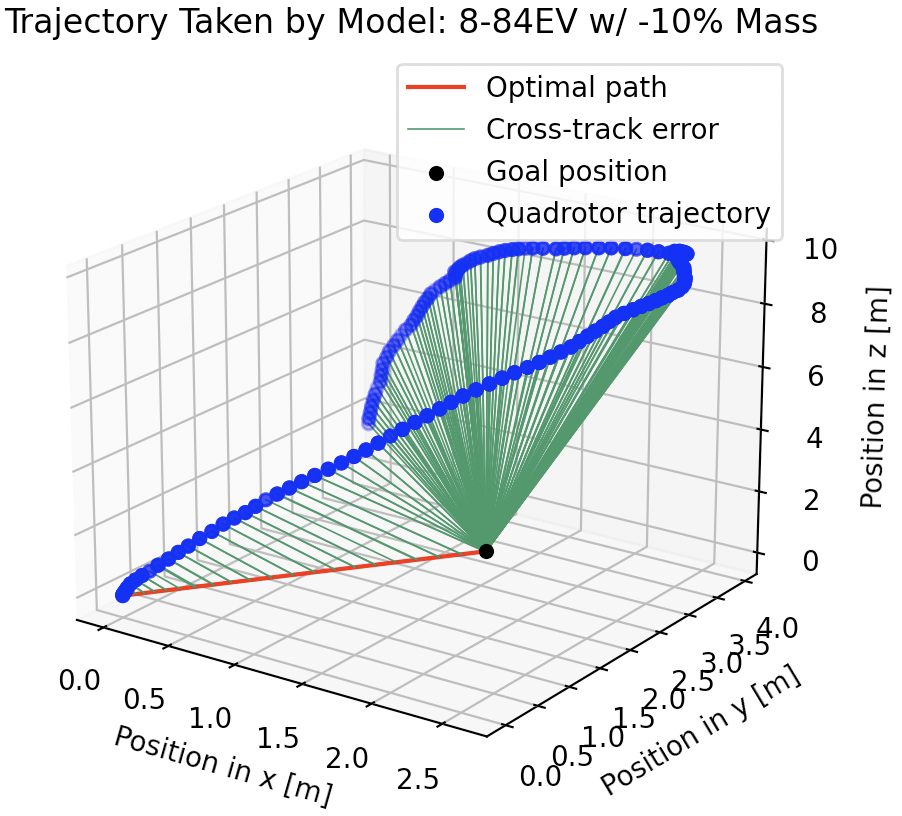
\includegraphics[width=\textwidth]{figures/5_/Testing/ppo_test_robust-10-884EV1.png}
         \caption{Trajectory of 8-84EV -10\% Mass.}
         \label{fig:testing_robust-10_ppo884EV1}
     \end{subfigure} 
     \hfill 
    \begin{subfigure}[b]{0.49\textwidth}
         \centering
         \captionsetup{justification=centering}
         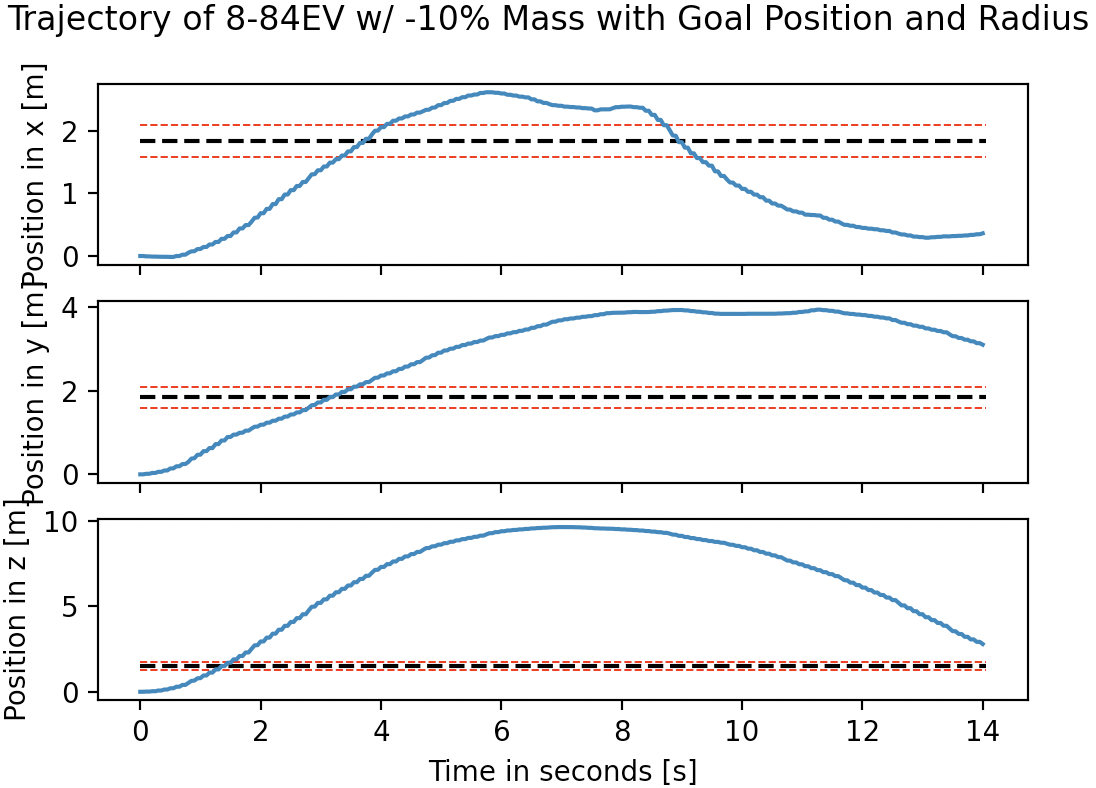
\includegraphics[width=\textwidth]{figures/5_/Testing/ppo_test_robust-10-884EV2.png}
         \caption{Trajectory of 8-84EV -10\% Mass, decomposed in $x$, $y$, $z$.}
         \label{fig:testing_robust-10_ppo884EV2}
     \end{subfigure} 
     \hfill \\[1mm]
    \begin{subfigure}[b]{0.48\textwidth}
         \centering
         \captionsetup{justification=centering}
         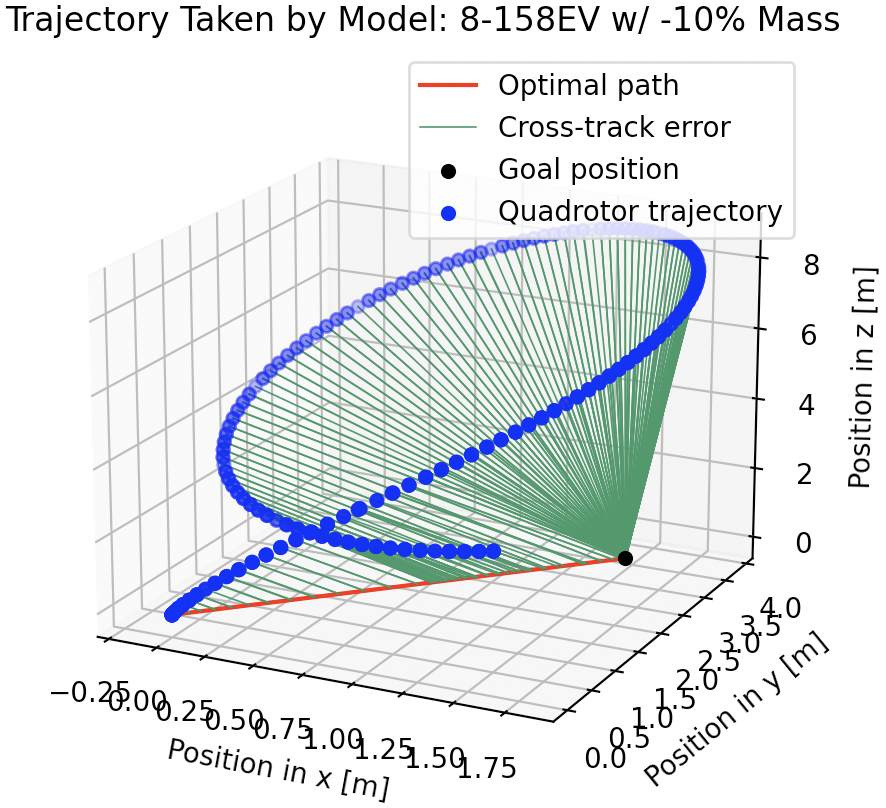
\includegraphics[width=\textwidth]{figures/5_/Testing/ppo_test_robust-10-8158EV1.png}
         \caption{Trajectory of 8-158EV -10\% Mass.}
         \label{fig:testing_robust-10_ppo8158EV1}
     \end{subfigure} 
     \hfill 
     \begin{subfigure}[b]{0.49\textwidth}
         \centering
         \captionsetup{justification=centering}
         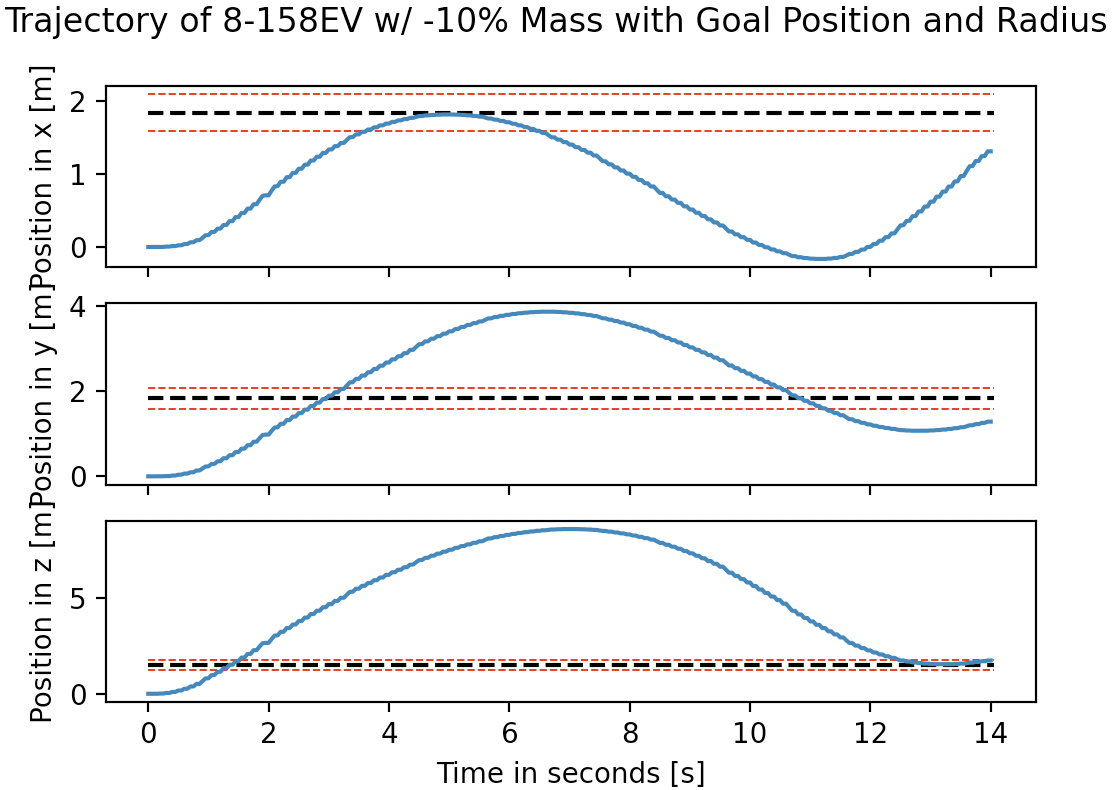
\includegraphics[width=\textwidth]{figures/5_/Testing/ppo_test_robust-10-8158EV2.png}
         \caption{Trajectory of 8-158EV -10\% Mass, decomposed in $x$, $y$, $z$.}
         \label{fig:testing_robust-10_ppo8158EV2}
     \end{subfigure} 
     \hfill \\[1mm]
    \begin{subfigure}[b]{0.48\textwidth}
         \centering
         \captionsetup{justification=centering}
         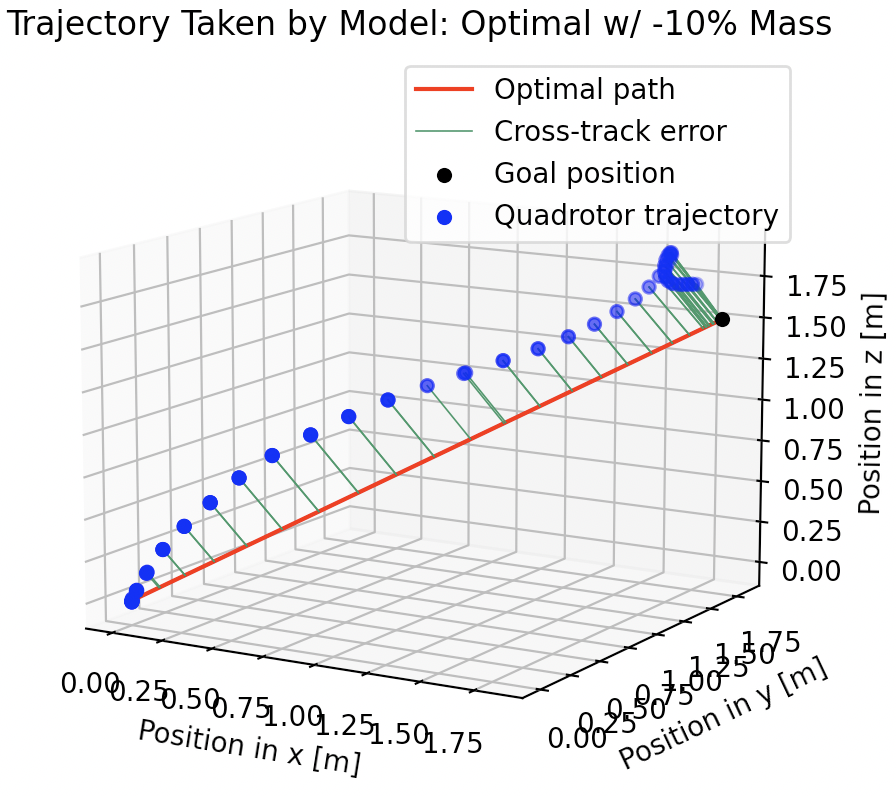
\includegraphics[width=\textwidth]{figures/5_/Testing/ppo_test_robust-10-Optimal1.png}
         \caption{Trajectory of Optimal -10\% Mass.}
         \label{fig:testing_robust-10_ppoOptimal1}
     \end{subfigure} 
     \hfill 
     \begin{subfigure}[b]{0.49\textwidth}
         \centering
         \captionsetup{justification=centering}
         \includegraphics[width=\textwidth]{figures/5_/Testing/ppo_test_robust-10-Optimal2.png}
         \caption{Trajectory of Optimal -10\% Mass, decomposed in $x$, $y$, $z$.}
         \label{fig:testing_robust-10_ppoOptimal2}
     \end{subfigure}
    \captionsetup{justification=centering}
    \caption{Robustness test run no. 100 -10\% mass for 8-84EV, 8-158EV and Optimal PPO models.}
     \label{fig:5_testing_robust-10_PPO}
\end{figure}


\subsubsection{Brief Summary}
We have seen that the effect of a higher entropy coefficient and value coefficient is beneficial to tested performance, as expected from training. We also confirmed that a batch size of 8000 was good, seen for example in models 4-84EV and 8-84EV.

Otherwise, we obtained some interesting results for the number of optimisation epochs and minibatches, where increasing these improved the chances of reaching the goal, but also led to increased anomalies which lowered the average return and increased RMSE. Thus, we have our most consistent model, 8-84EV, and our most goal-effective model, 8-158EV.

Next, we observed that our Optimal model did not require any hyperparameter tuning and had no troubles in the waypoint navigation task with a perfect 100\% goal rate.

In the robustness tests, we observed that the models \six and \ten struggled only with reaching the goal height in the +10\% mass case but had a drastic overshoots in all axes for the -10\% case. However, the Optimal model was relatively robust, being barely below the goal height in  +10\% mass case and managing a 100\% goal rate in the -10\% case.


\section{DDPG versus PPO}
After a relatively long presentation of results, the best models for DDPG and PPO are summarised in Table \ref{table:5_DDPG_PPO_bestModels}.
\begin{table}[hbt]
    \centering
    \begin{tabular}{||M{2.3cm}||M{2.5cm}|M{2.5cm}|M{2.5cm}||}
    \hline
        Model & Adjusted Goal Rate & Adjusted Avg. Return & Adjusted Avg. RMSE \\\hline\hline
        \textbf{DDPG} &  &   & \\\hline
        Modified & 100 & 0.267 & 0.025   \\\hline\hline
        \textbf{PPO} &   &   & \\\hline
        8-158EV &   85.9  & -0.133 & 0.044 \\\hline
        Optimal &   100  & 0.429 & 0.018 \\\hline
    \end{tabular}
    \caption{The best models for DDPG and PPO, where the results neglect outliers.}
    \label{table:5_DDPG_PPO_bestModels}
\end{table}
This table shows that our Optimal PPO model is the best model overall, which can be further confirmed by comparing its trajectory in Figure \ref{fig:testing_ppoOptimal2} to Modified's trajectory in \cref{fig:testing_ddpgModified2}. Next, DDPG's Modified model easily outperforms model 8-158EV, which has a significantly poorer performance compared to the two best models. 

In addition, we have seen that the PPO models are much quicker to train compared to the DDPG models, taking on average about a third of the total DDPG time to peak performance. This being said, the yield on the additional training time does pay off, resulting in overwhelming success in training for DDPG compared to PPO. The reason for this was that models for DDPG converge to global optima, while PPO models approach some local optima before diverging. The reasons for this will be discussed in Section \ref{sec:6_underperformance_divergence_PPO}. 

The success in training for DDPG was also seen through its test results, with the Original and Modified models dominating PPO in terms of average return and goal rates, and similar in terms of RMSE with PPO's most consistent model, 8-84EV. The reason for this is due to the local optimum strategy of the PPO models -- a trajectory that overshoots the goal height and doing some loop in order to reach the goal -- compared to the direct, globally optimum approach in the DDPG models.

For the robustness tests, the Modified model performed better in the +10\% mass case compared to the PPO models, but surprisingly performed worse than model 8-158EV in the -10\% mass case. For this situation, the overshoot caused by the lower mass was manageable by the PPO loop strategy, while the DDPG model could not adapt in the unfamiliar state space.

However, the wildcard performance of PPO's Optimal model is a testament to the potential of PPO. This model was in all regards optimal, being relatively exceptional in the robustness tests compared to the other models and the only model capable of reaching the goal in the -10\% case, let alone with a 100\% goal rate. As such, from the results in this project, we can conclude that training a DDPG agent is overall easier and more stable, while the potential performance of a PPO agent is unmatched.

